% !TEX program = xelatex
% IA712 - Project B: Autonomous Search and Rescue - rapport 10 pages (FR)
\documentclass[11pt,a4paper]{article}

\usepackage{amsmath}
\usepackage{fontspec}                 % XeLaTeX; defaults to Latin Modern (ships with TeX Live)
\usepackage[a4paper,margin=2cm]{geometry}
\usepackage{graphicx}
\graphicspath{{img/}}
\usepackage{xcolor}
\usepackage{tikz}
\usetikzlibrary{arrows.meta,positioning,shapes.geometric,fit,backgrounds,calc,decorations.pathreplacing}
\usepackage{booktabs}
\usepackage{enumitem}
\setlist{nosep,leftmargin=1.2em}
\usepackage{caption}
\captionsetup{font=small,labelfont=bf,skip=3pt}
\usepackage{subcaption}
\usepackage{titlesec}
\titlespacing*{\section}{0pt}{6pt}{3pt}
\titlespacing*{\subsection}{0pt}{4pt}{2pt}
\titleformat{\section}{\normalfont\large\bfseries\color{nccblue}}{\thesection}{0.5em}{}
\titleformat{\subsection}{\normalfont\normalsize\bfseries}{\thesubsection}{0.5em}{}
\usepackage[colorlinks=true,linkcolor=nccblue,citecolor=nccblue,urlcolor=nccblue]{hyperref}
% keep figures near their text instead of letting them pile up at the end
\usepackage[section]{placeins}
\renewcommand{\topfraction}{0.92}
\renewcommand{\bottomfraction}{0.85}
\renewcommand{\textfraction}{0.06}
\renewcommand{\floatpagefraction}{0.72}
\setcounter{topnumber}{3}\setcounter{bottomnumber}{2}\setcounter{totalnumber}{5}

% -- theme colors --
\definecolor{nccblue}{HTML}{1F4E79}
\definecolor{nccsky}{HTML}{1F6FEB}
\definecolor{nccorange}{HTML}{FB8500}
\definecolor{nccgreen}{HTML}{2DA44E}
\definecolor{nccred}{HTML}{D1242F}
\definecolor{nccgray}{HTML}{EEF1F5}
\definecolor{nccdark}{HTML}{222831}

% -- tikz styles --
\tikzset{
  box/.style={rounded corners=2pt,draw=nccblue,fill=nccgray,align=center,inner sep=3pt,font=\scriptsize,minimum height=7mm,text width=22mm},
  proc/.style={box,fill=white},
  phase1/.style={box,fill=nccsky!15,draw=nccsky},
  phase2/.style={box,fill=nccorange!15,draw=nccorange},
  btnode/.style={box,fill=nccblue!12,draw=nccblue},
  io/.style={box,fill=nccgreen!12,draw=nccgreen,rounded corners=6pt},
  ar/.style={-{Latex[length=2mm]},draw=nccdark!70,semithick},
  arl/.style={ar,font=\tiny,inner sep=1pt},
}

\newcommand{\head}[1]{\par\smallskip\noindent\textbf{\color{nccblue}#1}\par}

\begin{document}
\sloppy

% =================== TITLE BLOCK ===================
\begin{center}
  {\LARGE\bfseries\color{nccblue} Recherche et sauvetage autonomes}\\[2pt]
  {\large Projet B - IA712 Robotique mobile, projet final}\\[3pt]
  {\normalsize Équipe~\textbf{RobotZ}}\\[4pt]
  {\small ROS\,2 Humble $\cdot$ Ignition Gazebo Fortress $\cdot$ TurtleBot~4 $\cdot$ Nav2 $\cdot$ slam\_toolbox $\cdot$ BehaviorTree.CPP}\\[4pt]
  {\footnotesize Dépôt : \url{https://github.com/YiZeems/autonomous-search-and-rescue}}
\end{center}

\vspace{-2pt}
{\footnotesize
\begin{center}
\begin{tabular}{@{}llll@{}}
\toprule
\textbf{Membre} & \textbf{Courriel} & \textbf{Membre} & \textbf{Courriel}\\
\midrule
Julien GIMENEZ & \texttt{julien.gimenez@telecom-paris.fr} & Paul CINTRA & \texttt{paul.cintra@telecom-paris.fr}\\
Hugo FANCHINI  & \texttt{hugo.fanchini@telecom-paris.fr}  & Yimou ZHANG & \texttt{yimou.zhang@telecom-paris.fr}\\
\bottomrule
\end{tabular}
\end{center}}

\noindent\fcolorbox{nccblue}{nccblue!6}{\parbox{\dimexpr\linewidth-2\fboxsep-2\fboxrule}{%
\small\textbf{Résumé.}\ Un unique TurtleBot~4 explore de façon autonome une arène de catastrophe
cloisonnée et inconnue, construit une carte par SLAM et localise quatre «~victimes~» (AprilTags) en
projetant les détections caméra dans le repère global \texttt{map} à l'aide de \texttt{tf2}. La prise
de décision repose sur un \emph{Behavior Tree} (et non une FSM, comme exigé~[1]) qui orchestre une
\textbf{mission en deux phases} : exploration par frontières, puis inspection des pièces déduites de la
carte. Le run autonome final atteint \textbf{97,35\,\% de couverture et 4/4 victimes} en un seul clic.
Ce rapport présente l'architecture du système, les fondements théoriques, le cheminement
décisionnel de l'équipe à travers trois runs représentatifs et les enseignements tirés.}}

% =================== 1. INTRODUCTION ===================
\section{Énoncé du problème et exigences}
La robotique de recherche et sauvetage pose une question simple mais exigeante : lorsqu'un
environnement est trop dangereux pour des humains - un bâtiment effondré, un sous-sol inondé, une zone
d'accident nucléaire - un robot peut-il y entrer seul, comprendre un espace qu'il n'a jamais vu et en
rapporter la seule information qui compte, à savoir \emph{où se trouvent les victimes}~? Ce projet est
une réponse simulée et autonome à cette question, et une synthèse de l'ensemble du projet IA712 : il
relie SLAM, exploration autonome, navigation et prise de décision en un système unique qui se lance
d'une seule commande et ne requiert aucune intervention humaine.

Le scénario~[1] place un robot dans une zone de catastrophe simulée où les humains ne peuvent aller.
Le robot doit \emph{explorer de façon autonome} un environnement inconnu, \emph{localiser les victimes}
(AprilTags) et \emph{rapporter leurs coordonnées} dans un repère global. Ce qui rend la tâche
intéressante, c'est précisément que rien n'est connu à l'avance : le robot n'a pas de carte, il ignore
combien de pièces existent et où se trouvent les victimes, et il doit décider \emph{par lui-même} où
aller ensuite, quand il en a vu assez et quand la mission est terminée. L'énoncé fixe les contraintes
que nous satisfaisons :

\smallskip
{\footnotesize
\begin{tabular}{@{}p{0.30\linewidth}p{0.66\linewidth}@{}}
\toprule
\textbf{Exigence~[1]} & \textbf{Comment \texttt{bl} la satisfait}\\
\midrule
Exploration autonome (frontières / RRT), \emph{sans intervention humaine} & Exploration par frontières (Yamauchi~[2]) avec sélection par gain d'information~[3], cadencée par le BT\\
Qualité de la carte, fermeture de boucle & \texttt{slam\_toolbox} async avec fermeture de boucle~[4]\\
Détection caméra, projection vers \texttt{map} via \texttt{tf2} & \texttt{apriltag\_ros} (tag36h11)~[7] $\to$ \texttt{victim\_registry} projette caméra$\to$\texttt{map} (TF2)~[8]\\
Carte $>90\,\%$ de la zone & \textbf{97,35\,\%}\\
Carte finale annotée de toutes les positions des victimes & carte annotée + 4 victimes, Fig.~\ref{fig:results}\\
Décision = Behavior Tree, \emph{pas} de FSM & BehaviorTree.CPP~v3~[6]\\
Lancement en un clic & \texttt{ros2 launch rescue\_bringup bringup\_tb4.launch.py}\\
Bonus : couverture glouton vs.\ gain d'information & benchmark quantitatif ($n{=}3$), \S\ref{sec:concepts}\\
\bottomrule
\end{tabular}}

\head{Le système en un coup d'œil.} L'arène est un bâtiment cloisonné de quatre pièces
(\texttt{rescue\_arena}) avec une AprilTag «~victime~» sur un mur extérieur de chaque pièce. Le robot
est un \textbf{TurtleBot~4} (base Create~3, RPLIDAR~A1M8, caméra OAK-D) simulé sous \textbf{Ignition
Gazebo Fortress}. À partir d'un seul lancement, le robot cartographie le bâtiment par SLAM, visite de
façon autonome chaque pièce, détecte les quatre tags, les projette dans le repère \texttt{map} et
s'arrête sur une carte annotée et propre - \emph{sans} connaissance préalable des pièces ni des
positions des victimes. Les sections suivantes décrivent l'architecture, les concepts qu'elle
applique, et comment nous y sommes parvenus.

% =================== 2. ARCHITECTURE ===================
\section{Architecture du système}
L'espace de travail est découpé en \textbf{quatre paquets ROS\,2} afin que les quatre membres puissent
travailler en parallèle : \texttt{rescue\_bringup} (lancement + configs), \texttt{rescue\_robot}
(«~mégapaquet~» Python : exploration, perception, navigation/inspection, résultats), \texttt{rescue\_world}
(mondes Ignition + cibles AprilTag) et \texttt{rescue\_decision} (le Behavior Tree en C++). La
Fig.~\ref{fig:arch} est le schéma système détaillé exigé par~[1].

Ce découpage est délibéré. Une séparation nette entre \emph{ce que le robot perçoit} (SLAM, perception),
\emph{ce qu'il fait} (exploration, navigation, inspection), \emph{où il agit} (le monde simulé) et
\emph{comment il décide} (le Behavior Tree) a permis à quatre personnes de travailler en parallèle sur
leurs propres branches sans se gêner, et a maintenu chaque composant testable isolément - nous pouvions
exercer le Behavior Tree, le registre des victimes et la visualisation RViz contre de légers publieurs
factices, bien avant que la pile Gazebo complète n'existe. Tout aussi important, la conception trace une
frontière nette entre \emph{politique} et \emph{mécanisme} : le Behavior Tree décide \emph{quelle} phase
doit s'exécuter et \emph{quand} passer à la suivante, tandis que les nœuds Python sont de purs
exécutants qui ignorent tout de la mission globale. C'est cette frontière qui rend le système facile à
raisonner, et c'est ce que déploient les deux sections suivantes : d'abord les concepts sur
lesquels reposent les mécanismes, puis la mission que la politique assemble à partir d'eux.

\begin{figure}[htbp]
\centering
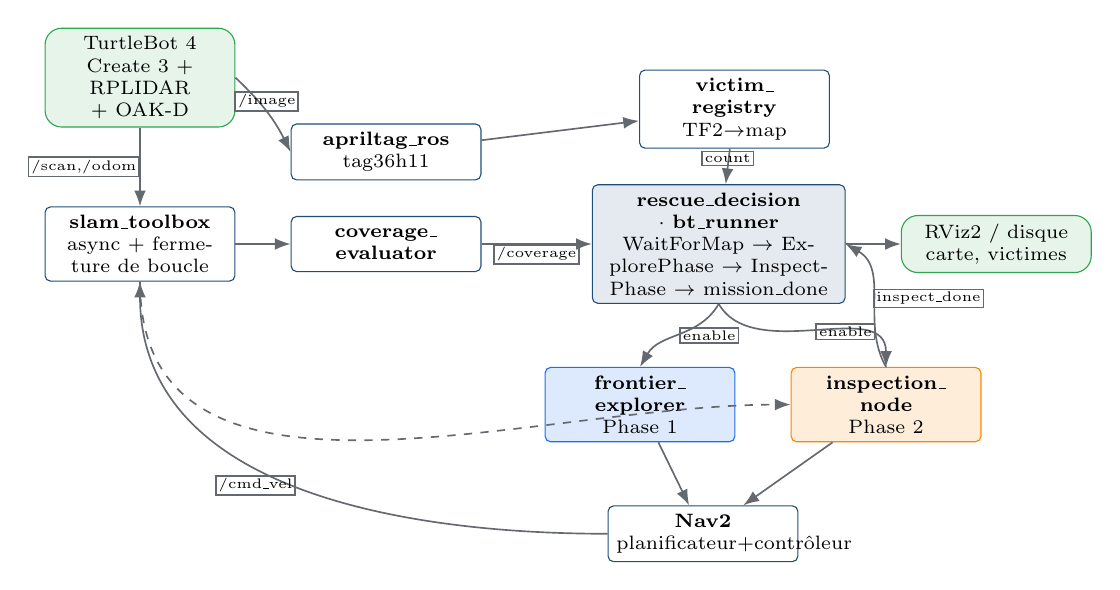
\begin{tikzpicture}[node distance=4.5mm and 7mm]
  \node[io] (robot) {TurtleBot~4\\\scriptsize Create~3 + RPLIDAR + OAK-D};
  \node[proc,below=10mm of robot] (slam) {\textbf{slam\_toolbox}\\\scriptsize async + fermeture de boucle};
  \node[proc,right=of slam] (metric) {\textbf{coverage\_}\\\textbf{evaluator}};
  \node[proc,above=of metric] (april) {\textbf{apriltag\_ros}\\\scriptsize tag36h11};
  \node[btnode,right=14mm of metric,text width=30mm] (bt) {\textbf{rescue\_decision $\cdot$ bt\_runner}\\\scriptsize WaitForMap $\to$ ExplorePhase $\to$ InspectPhase $\to$ mission\_done};
  \node[phase1,below=8mm of bt,xshift=-10mm] (explore) {\textbf{frontier\_}\\\textbf{explorer}\\\scriptsize Phase 1};
  \node[phase2,right=of explore] (inspect) {\textbf{inspection\_}\\\textbf{node}\\\scriptsize Phase 2};
  \node[proc,below=8mm of explore,xshift=8mm] (nav) {\textbf{Nav2}\\\scriptsize planificateur+contrôleur};
  \node[proc,above=of bt,xshift=2mm] (reg) {\textbf{victim\_}\\\textbf{registry}\\\scriptsize TF2$\to$map};
  \node[io,right=of bt] (rviz) {RViz2 / disque\\\scriptsize carte, victimes};

  \draw[ar] (robot) -- node[arl,left]{/scan,/odom} (slam);
  \draw[ar] (robot.east) to[bend left=10] node[arl,above]{/image} (april.west);
  \draw[ar] (slam) -- (metric);
  \draw[ar] (april) -- (reg);
  \draw[ar] (metric) -- node[arl,below]{/coverage} (bt);
  \draw[ar] (bt.south) to[out=-120,in=60] node[arl,right]{enable} (explore.north);
  \draw[ar] (bt.south) to[out=-60,in=90] node[arl,right]{enable} (inspect.north);
  \draw[ar] (inspect.north) to[out=120,in=-30] node[arl,right]{inspect\_done} (bt.east);
  \draw[ar] (explore) -- (nav);
  \draw[ar] (inspect) -- (nav);
  \draw[ar] (nav.west) to[out=180,in=-90] node[arl,left]{/cmd\_vel} (slam.south);
  \draw[ar] (reg) -- node[arl,above]{count} (bt);
  \draw[ar] (bt) -- (rviz);
  \draw[ar,dashed] (slam) to[out=-90,in=180] (inspect.west);
\end{tikzpicture}
\caption{Architecture du système et flux de topics. Le Behavior Tree (\texttt{rescue\_decision}) est
l'\emph{orchestrateur} : il cadence l'explorateur de la Phase~1 et l'inspecteur de la Phase~2 via les
topics \texttt{/mission/*} ; les nœuds Python font le travail. Le SLAM alimente la carte vers
l'exploration, la couverture, Nav2 et l'inspection.}
\label{fig:arch}
\end{figure}

\noindent Les paquets et leurs responsabilités :
\begin{itemize}
\item \textbf{\texttt{rescue\_bringup}} - le point d'entrée \emph{en un clic}
(\texttt{bringup\_tb4.launch.py}) et toutes les configs (Nav2, SLAM, AprilTag). Un seul lancement
démarre la simulation, le SLAM, Nav2, la perception, l'explorateur/inspecteur et le Behavior Tree.
\item \textbf{\texttt{rescue\_robot}} - le «~mégapaquet~» Python : \texttt{exploration/}
(recherche de frontières + liste noire), \texttt{navigation/} (planificateur d'inspection + nœud),
\texttt{detection/} (registre/détecteur de victimes), \texttt{results/} (évaluateur de couverture +
exporteur de résultats) et des mocks de développement.
\item \textbf{\texttt{rescue\_world}} - l'arène Ignition Fortress (\texttt{rescue\_arena.sdf}) et les
cibles AprilTag en voxels. Une \emph{source unique} possède le placement des victimes, de sorte que la
carte et la vérité terrain ne divergent jamais.
\item \textbf{\texttt{rescue\_decision}} - le véritable exécuteur C++ \texttt{BehaviorTree.CPP\,v3}
(visualisable dans Groot), avec le XML de l'arbre de mission. C'est l'exigence «~décision = BT, pas de
FSM~».
\end{itemize}

\head{Pipeline de perception.} Les victimes sont des AprilTags \texttt{tag36h11} (l'énoncé exclut
explicitement toute détection humaine sophistiquée / YOLO). Une difficulté subtile : un tag à texture
PBR se rend \emph{blanc} sous Ogre2+Mesa, de sorte que \texttt{apriltag\_ros} ne voit rien ; nous
construisons chaque tag en \textbf{boîtes de voxels} avec un anneau blanc de zone calme autour du
marqueur natif $8{\times}8$ (un redimensionnement naïf en $10{\times}10$ détruit la zone calme et rend
le tag \emph{affiché mais indétectable}). Chaque détection fournit une transformée
\texttt{camera}$\to$\texttt{victim}\_$i$ ; \texttt{victim\_registry} la projette vers \texttt{map} via
TF2, déduplique par ID et persiste \texttt{results/victims.json} - l'exigence «~rapporter leurs
coordonnées dans le repère global~».

% =================== 3. THEORETICAL FOUNDATIONS ===================
\section{Fondements théoriques}\label{sec:concepts}
\head{SLAM et fermeture de boucle.} Le robot construit la carte en ligne avec \texttt{slam\_toolbox}
(SLAM par graphe de poses). La fermeture de boucle corrige la dérive
accumulée lorsque le robot ré-observe un lieu connu, gardant la carte globale cohérente lors de passages
répétés~[4,9].

\head{Exploration par frontières et gain d'information.} Une \emph{frontière} est la limite entre
les cellules libres et inconnues~[2]. La sélection gloutonne prend la frontière la plus proche ; la
sélection par \emph{gain d'information} maximise $\,g(f)=\mathrm{gain}(f)-\lambda\cdot\mathrm{cost}(f)\,$~[3],
où $\mathrm{cost}$ est la \emph{longueur du chemin Nav2} (pas euclidienne). Notre benchmark $n{=}3$
confirme la théorie : le gain d'information atteint $0{,}85\pm0{,}08$ de couverture (la seule au-dessus
de $90\,\%$) contre $0{,}72$ pour le glouton. \emph{Pourquoi} l'écart se creuse \emph{dans le temps}
(Fig.~\ref{fig:bench}) : le glouton, attiré par la frontière la plus proche, raffine la zone déjà ouverte
et repousse les pièces lointaines, donc plafonne ($\sim$67--70\,\%) ; le gain d'information préfère la
frontière qui révèle le plus d'inconnu \emph{par mètre} (une porte ouvrant une pièce entière), donc chaque
déplacement rapporte plus et la courbe franchit les $90\,\%$ - et comme le coût est la longueur de chemin
Nav2 (pas euclidienne), les murs sont pris en compte. Un ajout clé de robustesse est une \emph{liste noire de
frontières inaccessibles} indexée par une coordonnée monde quantifiée, de sorte qu'une frontière morte
ne soit jamais resélectionnée même lorsque l'origine de la grille se décale. Concrètement, une frontière
est blacklistée soit quand Nav2 échoue à l'atteindre, soit quand elle est re-sélectionnée \textbf{3 fois
de suite sans gain de couverture} (le cas courant dans notre arène) ; elle n'est alors plus jamais reproposée.

\begin{figure}[htbp]
\centering
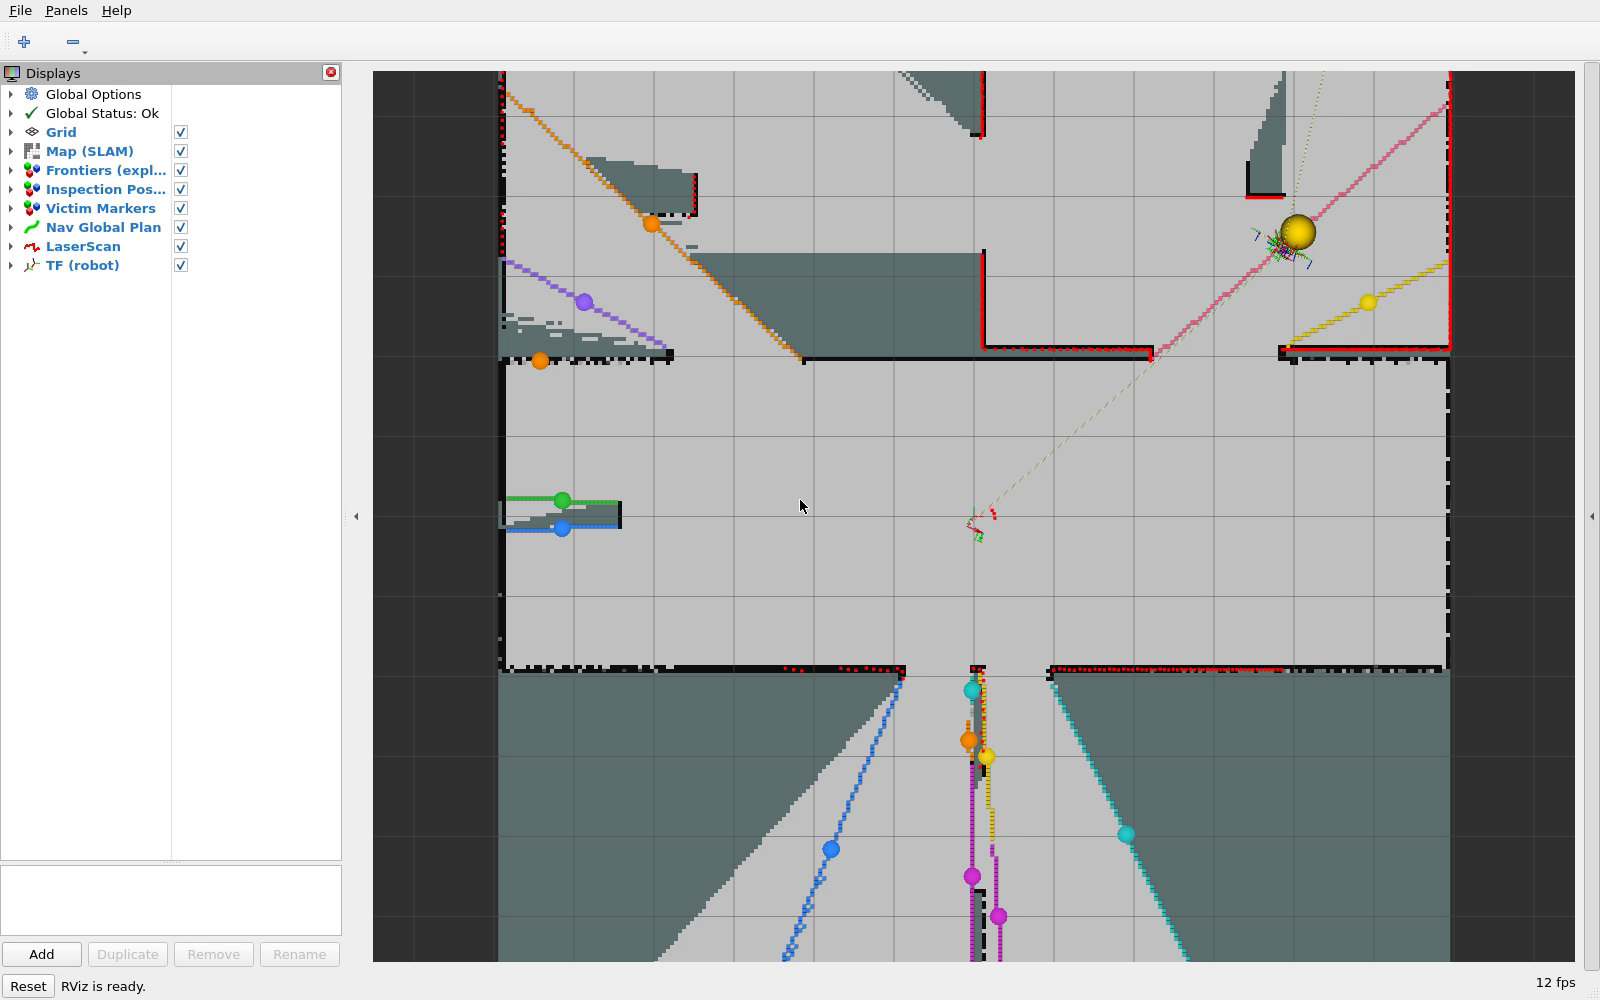
\includegraphics[width=0.72\linewidth]{rviz_frontiers}
\caption{Exploration par frontières dans RViz, forme et couleur de chaque élément :
\textbf{cubes colorés} = cellules de frontière (limite connu/inconnu), \textbf{une couleur par cluster}
(composante connexe) ; \textbf{sphères de même couleur} = centroïdes des clusters ; \textbf{grosse sphère
jaune} = frontière-but retenue ($g=\mathrm{gain}-\lambda\,\mathrm{cost}$) ; \textbf{ligne bleue} = plan
Nav2 ; \textbf{axes RVB} = robot (TF). Fond clair = libre, gris-bleu = inconnu, traits noirs/rouges = murs.}
\label{fig:rviz-frontiers}
\end{figure}

\head{Planification de chemin et contrôle.} Le planificateur global produit un chemin
géométrique ; le contrôleur local le suit. Nous avons comparé \emph{Dijkstra/NavFn} vs.\ \emph{A* (Smac)}~[9] :
dans une arène fortement cloisonnée, le robot se tient souvent à l'intérieur de la couche d'inflation, où
A* refuse de planifier («~start in lethal space~») ; NavFn le tolère et est conservé. Le contrôleur est
DWB (par échantillonnage).

\begin{figure}[htbp]
\centering
\begin{subfigure}{0.44\linewidth}\centering
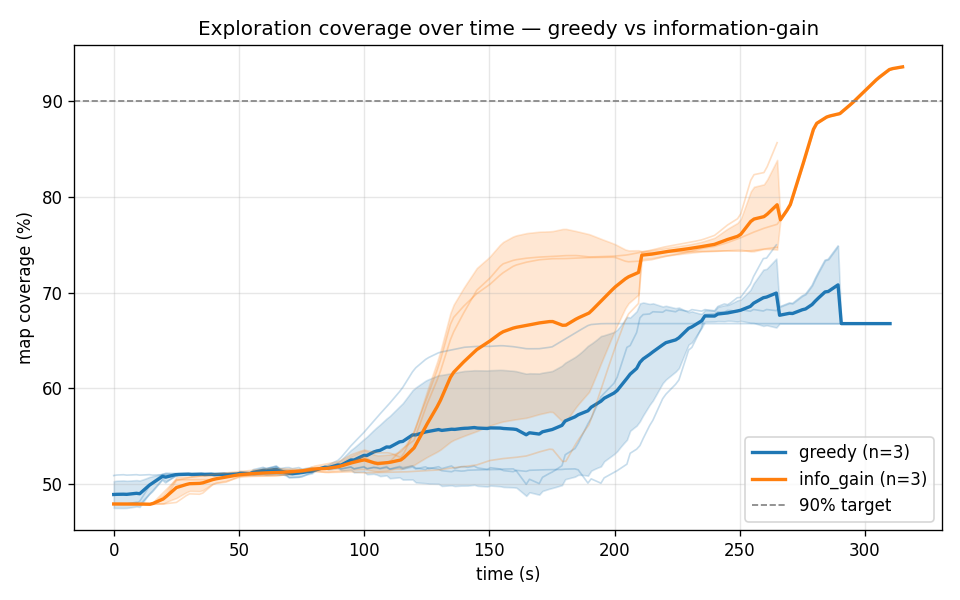
\includegraphics[width=\linewidth]{coverage_over_time}
\caption{Bonus ($n{=}3$) - couverture cartographique \emph{au fil du temps} : le \textbf{gain
d'information} (orange) atteint la cible 90\,\%, le \textbf{glouton} (bleu) plafonne $\sim$67--70\,\%.}
\end{subfigure}\hfill
\begin{subfigure}{0.53\linewidth}\centering\footnotesize
\begin{tabular}{@{}lll@{}}
\toprule
Planificateur & Propriété & Statut dans \texttt{bl}\\
\midrule
Dijkstra/NavFn & optimal, explore tout, tolérant & \textbf{choisi} (robuste)\\
A* (Smac) & heuristique, plus rapide, strict & testé, écarté ici\\
RRT & rapide, non optimal & perspective\\
\bottomrule
\end{tabular}
\par\smallskip
\emph{Pourquoi NavFn :} dans une arène cloisonnée, le départ est souvent dans la couche d'inflation ; A*
y abandonne, pas NavFn.
\end{subfigure}
\caption{Stratégie d'exploration (bonus) et comparaison des planificateurs globaux.}
\label{fig:bench}
\end{figure}

\head{Repères de coordonnées et TF2.} Une victime est détectée dans le repère \emph{camera} ; \texttt{tf2}
enchaîne $\text{camera}\to\text{victim}\_i\to\text{map}$ pour rapporter une position globale
(Fig.~\ref{fig:concepts}b), exactement l'exigence «~projeter les positions dans le repère global~»~[1,8].

\head{Behavior Trees vs.\ FSM.} L'énoncé interdit les FSM. Un BT est réactif et composable : une
\texttt{Sequence} avec mémoire tique ses enfants de gauche à droite, \emph{reprend} au nœud RUNNING et
n'avance que sur SUCCESS - une véritable séquence de phases plutôt que des transitions d'état codées à la
main~[6].

\begin{figure}[htbp]
\centering
\begin{subfigure}{0.47\linewidth}\centering
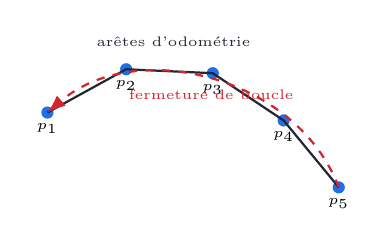
\begin{tikzpicture}[font=\scriptsize]
  \foreach \i/\x/\y in {1/0/0,2/1.0/0.55,3/2.1/0.5,4/3.0/-0.1,5/3.7/-0.95}{
     \fill[nccsky] (\x,\y) circle (2.2pt); \node[below=0.5pt,font=\tiny] at (\x,\y){$p_\i$};}
  \draw[nccdark,thick] (0,0)--(1.0,0.55)--(2.1,0.5)--(3.0,-0.1)--(3.7,-0.95);
  \node[font=\tiny,nccdark] at (1.6,0.9){arêtes d'odométrie};
  \draw[dashed,nccred,-{Latex},thick] (3.7,-0.95) to[bend right=55] node[below,font=\tiny,nccred]{fermeture de boucle} (0,0);
\end{tikzpicture}
\caption{Le SLAM est un graphe de poses : ré-observer un lieu connu ajoute une arête de \emph{fermeture de
boucle} qui corrige la dérive accumulée et garde la carte globale cohérente sur des passages répétés.}
\end{subfigure}\hfill
\begin{subfigure}{0.49\linewidth}\centering
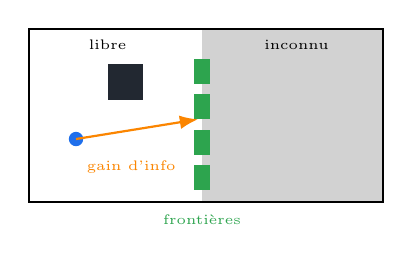
\begin{tikzpicture}[font=\scriptsize]
  \fill[gray!35] (2.2,0) rectangle (4.5,2.2);
  \draw[thick] (0,0) rectangle (4.5,2.2);
  \fill[nccdark] (1.0,1.3) rectangle (1.45,1.75);
  \foreach \y in {0.15,0.6,1.05,1.5} {\fill[nccgreen] (2.1,\y) rectangle (2.3,\y+0.32);}
  \fill[nccsky] (0.6,0.8) circle (2.6pt);
  \draw[-{Latex},nccorange,thick] (0.6,0.8)--(2.15,1.05);
  \node[font=\tiny] at (1.0,2.0){libre}; \node[font=\tiny] at (3.4,2.0){inconnu};
  \node[font=\tiny,nccgreen] at (2.2,-0.22){frontières}; \node[font=\tiny,nccorange] at (1.3,0.45){gain d'info};
\end{tikzpicture}
\caption{Une \emph{frontière} est la limite libre/inconnu (vert) ; le gain d'information sélectionne la
plus informative, notée par le coût de \emph{chemin} Nav2 (pas euclidien).}
\end{subfigure}
\caption{Deux concepts clés : SLAM par graphe de poses avec fermeture de boucle et
exploration par frontières avec gain d'information.}
\label{fig:keyconcepts}
\end{figure}

\begin{figure}[htbp]
\centering
\begin{subfigure}{0.49\linewidth}\centering
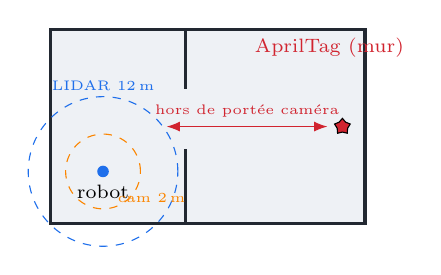
\begin{tikzpicture}[scale=0.95,every node/.style={font=\scriptsize}]
  % camera vs lidar gap
  \fill[nccgray] (0,0) rectangle (4.2,2.6);
  \draw[very thick,nccdark] (0,0) rectangle (4.2,2.6);
  \draw[very thick,nccdark] (1.8,2.6)--(1.8,1.8); \draw[very thick,nccdark] (1.8,0)--(1.8,1.0);
  \node[star,star points=5,fill=nccred,draw=black,inner sep=1.4pt] (tag) at (3.9,1.3) {};
  \node[right] at (2.6,2.35) {\color{nccred}AprilTag (mur)};
  \fill[nccsky] (0.7,0.7) circle (2.2pt); \node[below] at (0.7,0.65) {robot};
  \draw[dashed,nccsky] (0.7,0.7) circle (1.0cm); \node[nccsky] at (0.7,1.85){\tiny LIDAR 12\,m};
  \draw[nccorange,dashed] (0.7,0.7) circle (0.5cm); \node[nccorange] at (1.35,0.35){\tiny cam 2\,m};
  \draw[{Latex}-{Latex},nccred] (1.55,1.3)--(3.7,1.3) node[midway,above]{\tiny hors de portée caméra};
\end{tikzpicture}
\caption{Écart caméra-LIDAR : le LIDAR cartographie une pièce depuis l'embrasure, mais la caméra
n'approche jamais à 2\,m du tag mural $\Rightarrow$ l'exploration pure manque les victimes.}
\end{subfigure}\hfill
\begin{subfigure}{0.49\linewidth}\centering
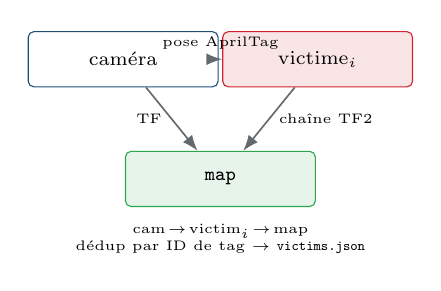
\begin{tikzpicture}[scale=0.95,every node/.style={font=\scriptsize}]
  \node[box,fill=white] (cam) at (0,0) {caméra};
  \node[box,fill=nccred!12,draw=nccred] (vic) at (2.6,0) {victime$_i$};
  \node[box,fill=nccgreen!12,draw=nccgreen] (map) at (1.3,-1.6) {\texttt{map}};
  \draw[ar] (cam) -- node[above,font=\tiny]{pose AprilTag} (vic);
  \draw[ar] (cam) -- node[left,font=\tiny]{TF}(map);
  \draw[ar] (vic) -- node[right,font=\tiny]{chaîne TF2}(map);
  \node[font=\tiny,align=center] at (1.3,-2.4){$\text{cam}\!\to\!\text{victim}_i\!\to\!\text{map}$\\dédup par ID de tag $\to$ \texttt{victims.json}};
\end{tikzpicture}
\caption{Projection TF2 d'une détection dans le repère global \texttt{map}.}
\end{subfigure}
\caption{Deux concepts clés derrière la mission.}
\label{fig:concepts}
\end{figure}

\head{La mission en deux phases.} L'exploration pure complète la \emph{carte} mais plafonne la détection
des victimes (Fig.~\ref{fig:concepts}a). Le remède est une seconde phase \emph{autonome} : à partir de la
carte qu'il vient de construire, \texttt{inspection\_node} dérive \emph{une pose par pièce découverte}
(face au mur le plus proche, alignée sur une cellule navigable, \emph{sans coordonnées de victimes}) ; le
robot s'y rend et balaie la caméra. L'arbre de mission BT est la \texttt{Sequence}
\textsf{WaitForMap\,$\to$\,ExplorePhase\,$\to$\,InspectPhase\,$\to$\,VictimsFound\,$\to$\,mission\_done}
(Fig.~\ref{fig:bt}).

\begin{figure}[htbp]
\centering
\begin{subfigure}{0.34\linewidth}\centering
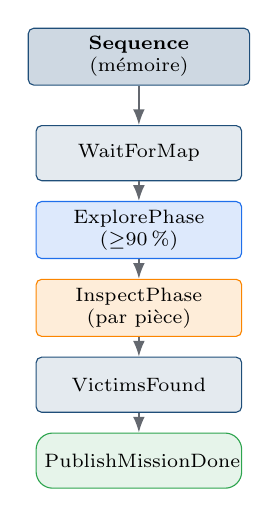
\begin{tikzpicture}[font=\scriptsize,node distance=3mm]
  \node[btnode,fill=nccblue!22,text width=26mm] (root) {\textbf{Sequence} (mémoire)};
  \node[btnode,below=5mm of root,text width=24mm] (n1) {WaitForMap};
  \node[phase1,below=2.5mm of n1,text width=24mm] (n2) {ExplorePhase ($\geq$90\,\%)};
  \node[phase2,below=2.5mm of n2,text width=24mm] (n3) {InspectPhase (par pièce)};
  \node[btnode,below=2.5mm of n3,text width=24mm] (n4) {VictimsFound};
  \node[io,below=2.5mm of n4,text width=24mm] (n5) {PublishMissionDone};
  \draw[ar] (root) -- (n1);
  \draw[ar] (n1) -- (n2); \draw[ar] (n2) -- (n3); \draw[ar] (n3) -- (n4); \draw[ar] (n4) -- (n5);
\end{tikzpicture}
\caption{Arbre de mission : une \texttt{Sequence} à mémoire qui reprend la phase RUNNING.}
\end{subfigure}\hfill
\begin{subfigure}{0.64\linewidth}\centering

\includegraphics[width=\linewidth]{algorithms_two_phase}
\caption{Les algorithmes à l'œuvre. \emph{À gauche :} exploration par frontières de la Phase~1 (chemin
bleu, objectifs de gain d'info verts). \emph{À droite :} inspection de la Phase~2 (chemin orange, poses
déduites de la carte) capturant les quatre victimes. Les murs sont dessinés par-dessus le chemin, qui se
faufile donc visiblement par les embrasures.}
\end{subfigure}
\caption{La mission en deux phases orchestrée par le Behavior Tree.}
\label{fig:bt}
\end{figure}

\head{Concepts \emph{appliqués} dans le projet.} Le Tableau~\ref{tab:concepts} associe chaque
concept à l'endroit où il est appliqué dans notre système.

\begin{table}[htbp]\centering\footnotesize
\begin{tabular}{@{}p{0.30\linewidth}p{0.66\linewidth}@{}}
\toprule
\textbf{Concept} & \textbf{Où il est appliqué dans \texttt{bl}}\\
\midrule
SLAM + fermeture de boucle & \texttt{slam\_toolbox} (async) : \texttt{/map} en ligne + TF \texttt{map}$\to$\texttt{odom}, fermeture de boucle sur les revisites\\
Exploration par frontières & \texttt{frontier\_explorer\_node} : limite libre/inconnu, liste noire indexée monde\\
Gain d'information (bonus) & sélection de frontières par gain d'info ; benchmark quantitatif vs.\ glouton ($n{=}3$)\\
Planification de chemin & planificateur global Nav2 - NavFn (Dijkstra) conservé ; A* (Smac) comparé\\
Contrôle local & contrôleur Nav2 DWB (scoring de trajectoires par échantillonnage)\\
Repères de coordonnées / TF2 & \texttt{victim\_registry} : projection caméra$\to$\texttt{victim}$_i\to$\texttt{map}\\
Behavior Trees (décision) & \texttt{rescue\_decision} (BT.CPP~v3) : orchestration de la mission en deux phases\\
\bottomrule
\end{tabular}
\caption{Les concepts clés, et exactement où chacun est appliqué dans le projet.}
\label{tab:concepts}
\end{table}

% =================== 4. DECISION JOURNEY ===================
\section{Cheminement décisionnel : trois runs représentatifs}
Les chiffres phares - 97\,\% de couverture, quatre victimes, un clic - masquent une route longue et
instructive. Rien n'est venu d'un coup : presque chaque capacité que nous tenons aujourd'hui pour acquise
a été, à un moment, un run qui faisait la mauvaise chose pour une raison que nous ne comprenions pas
encore. Nous avons tenu un journal décisionnel écrit au format \emph{Problème $\to$ Investigation $\to$
Décision $\to$ Pourquoi}, et l'habitude la plus utile qu'il nous a apprise a été de \emph{mesurer avant
de prescrire} - de laisser un journal d'événements ou une métrique, plutôt qu'une intuition, nous dire ce
qui n'allait réellement pas. Trois runs distillent cette histoire ; chacun est rapporté ci-dessous comme
ce qui a \emph{bloqué} et ce que nous avons \emph{amélioré}, et la Fig.~\ref{fig:journey} en est la
synthèse sur une page.

\head{Run 1 - exploration autonome pure (v20--v22).} Notre premier système complet faisait la chose
évidente : exploration par frontières pilotant Nav2, avec \texttt{slam\_toolbox} construisant la carte
en dessous. Cela marchait, au sens où il cartographiait de façon autonome environ quatre-vingt-dix pour
cent du bâtiment - mais il ne trouvait toujours qu'environ deux des quatre victimes, et pendant longtemps
nous ne voyions pas pourquoi. La réponse s'est révélée géométrique plutôt qu'algorithmique : un LIDAR de
douze mètres cartographie confortablement une pièce depuis son embrasure, donc un robot qui optimise la
\emph{couverture} n'a aucune raison de s'approcher d'un mur, alors que la caméra ne reconnaît un tag qu'à
deux mètres environ. L'exploration était donc \emph{complète} et la détection \emph{structurellement
incomplète} en même temps. En chemin, ce run nous a aussi enseigné deux leçons tranchantes - une frontière
que le planificateur ne peut jamais atteindre piégera le robot dans une boucle infinie tant qu'elle n'est
pas mise en liste noire, et un facteur temps réel assez bas pour affamer le renderer GPU de la caméra
arrêtera silencieusement la détection alors que les métadonnées de la caméra continuent de circuler et
masquent le défaut. Nous avons quitté ce run avec une carte propre, une autonomie fiable et un diagnostic
clair de ce qui manquait encore.

\head{Run 2 - deux phases, orchestré par BT (v32).} Le correctif a découlé directement de ce diagnostic :
si le robot ne s'approche pas des murs en explorant, donnons-lui une seconde raison de le faire. Nous
avons ajouté une phase d'\emph{inspection} qui lit la carte fraîchement construite, dérive une pose par
pièce découverte à environ 1,3\,m du mur le plus proche - dans la portée de la caméra, mais en utilisant
uniquement la carte et jamais les positions des victimes - et visite chacune tour à tour en balayant la
caméra. Surtout, nous avons aussi promu le Behavior Tree d'un superviseur passif qui se contentait de
surveiller la métrique de couverture en véritable \emph{orchestrateur} de la mission, cadençant
exploration et inspection en séquence ; c'est ce qui rend le système conforme à l'exigence «~décision par
Behavior Tree, pas de FSM~» sur le fond et pas seulement sur le nom. Le résultat fut la percée que nous
cherchions : \textbf{quatre victimes sur quatre et 97\,\% de couverture} en un seul run continu et
entièrement autonome.

\head{Run 3 - le livrable final.} La mission fonctionnant, le dernier run a consisté à transformer un
résultat en un livrable fiable et reproductible. Nous nous sommes d'abord demandé si nous pouvions
simplement faire tourner la simulation plus vite : pousser le facteur temps réel à 1,5 finissait bien
plus tôt, mais laissait moins de temps à la caméra pour se stabiliser à chaque pose et nous ramenait
discrètement à trois victimes sur quatre, en plus de stresser le GPU - nous avons donc gardé le facteur
plus lent et fiable, petit rappel que pour un livrable, la répétabilité l'emporte sur la vitesse. Nous
avons ensuite réglé un ensemble de problèmes de présentation qui, sans affecter le comportement du robot,
affectaient la capacité d'un lecteur à \emph{faire confiance} aux figures : la trajectoire dans le repère
carte est désormais tracée avec les murs peints \emph{par-dessus}, de sorte que le chemin n'apparaît
jamais que dans l'espace libre et se faufile visiblement par chaque embrasure (nous avons vérifié qu'aucun
de ses 568 segments ne traverse un mur) ; la carte d'occupation est rendue avec la bonne orientation
verticale, ce qui était la vraie raison pour laquelle une figure antérieure \emph{donnait l'impression}
que le robot traversait les murs ; et les fichiers de résultats de chaque run sont tronqués au démarrage,
si bien que les courbes d'un run ne s'empilent plus sur celles d'un autre. Le travail de robustesse qui
permet à l'inspection de récupérer une pose inatteignable sur la machine d'un coéquipier
(\S\ref{sec:concepts}) a aussi atterri ici. Le résultat est le run sur lequel s'appuie tout ce rapport :
\textbf{quatre victimes sur quatre, environ 97\,\% de couverture}, une carte annotée propre, une
trajectoire enregistrée et une capture HD des algorithmes RViz en direct - une source unique et
reproductible pour chaque figure présentée.

\begin{figure*}[t]
\centering
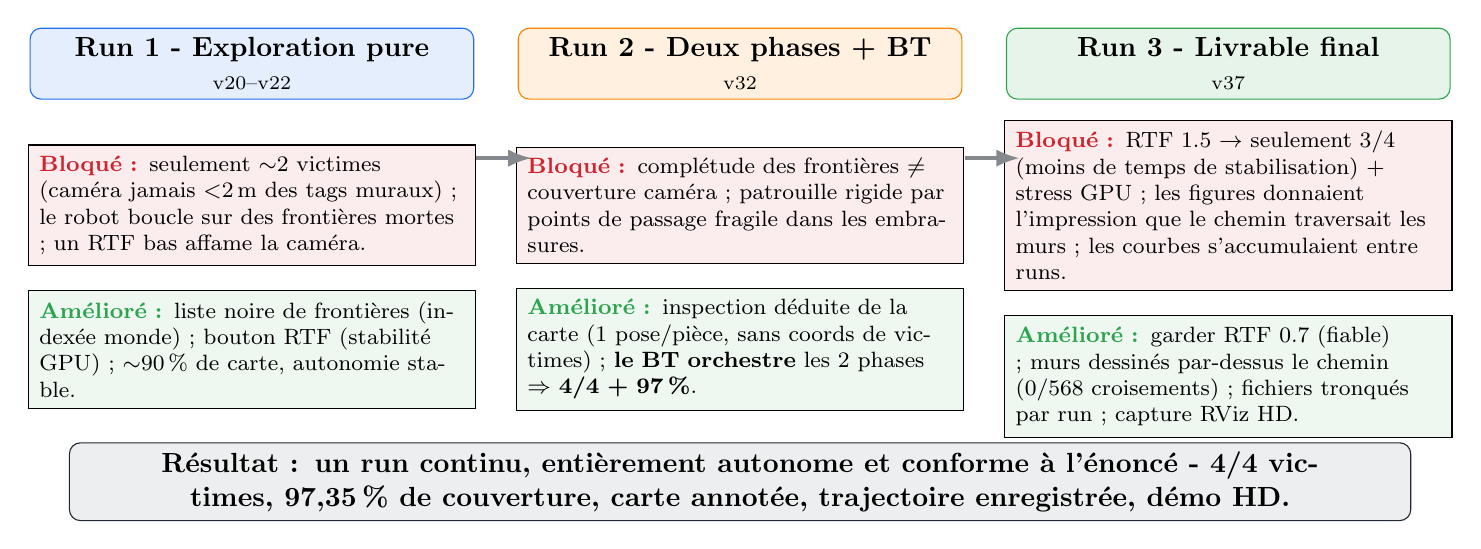
\begin{tikzpicture}[font=\footnotesize,node distance=3mm]
\definecolor{c1}{HTML}{1F6FEB}\definecolor{c2}{HTML}{FB8500}\definecolor{c3}{HTML}{2DA44E}
% three columns
\foreach \i/\x/\c/\title/\ver in {1/0/c1/{Run 1 - Exploration pure}/{v20–v22}, 2/6.2/c2/{Run 2 - Deux phases + BT}/{v32}, 3/12.4/c3/{Run 3 - Livrable final}/{v37}} {
  \node[draw=\c,fill=\c!12,rounded corners,text width=5.4cm,minimum height=8mm,align=center,font=\bfseries] (h\i) at (\x+2.7,5.2) {\title\\\normalfont\scriptsize \ver};
}
% Run1 body
\node[draw,fill=nccred!8,text width=5.4cm,align=left,inner sep=4pt] (b0) at (2.7,3.4)
 {\textbf{\color{nccred}Bloqué :} seulement $\sim$2 victimes (caméra jamais $<$2\,m des tags muraux) ; le robot boucle sur des frontières mortes ; un RTF bas affame la caméra.};
\node[draw,fill=nccgreen!8,text width=5.4cm,align=left,below=of b0,inner sep=4pt] (i0)
 {\textbf{\color{nccgreen}Amélioré :} liste noire de frontières (indexée monde) ; bouton RTF (stabilité GPU) ; $\sim$90\,\% de carte, autonomie stable.};
% Run2 body
\node[draw,fill=nccred!8,text width=5.4cm,align=left,inner sep=4pt] (b1) at (8.9,3.4)
 {\textbf{\color{nccred}Bloqué :} complétude des frontières $\neq$ couverture caméra ; patrouille rigide par points de passage fragile dans les embrasures.};
\node[draw,fill=nccgreen!8,text width=5.4cm,align=left,below=of b1,inner sep=4pt] (i1)
 {\textbf{\color{nccgreen}Amélioré :} inspection déduite de la carte (1 pose/pièce, sans coords de victimes) ; \textbf{le BT orchestre} les 2 phases $\Rightarrow$ \textbf{4/4 + 97\,\%}.};
% Run3 body
\node[draw,fill=nccred!8,text width=5.4cm,align=left,inner sep=4pt] (b2) at (15.1,3.4)
 {\textbf{\color{nccred}Bloqué :} RTF~1.5 $\to$ seulement 3/4 (moins de temps de stabilisation) + stress GPU ; les figures donnaient l'impression que le chemin traversait les murs ; les courbes s'accumulaient entre runs.};
\node[draw,fill=nccgreen!8,text width=5.4cm,align=left,below=of b2,inner sep=4pt] (i2)
 {\textbf{\color{nccgreen}Amélioré :} garder RTF~0.7 (fiable) ; murs dessinés par-dessus le chemin (0/568 croisements) ; fichiers tronqués par run ; capture RViz HD.};
\node[draw=nccdark,fill=nccdark!8,rounded corners,text width=16.8cm,align=center,below=4mm of i1,font=\bfseries] (res)
 {Résultat : un run continu, entièrement autonome et conforme à l'énoncé - 4/4 victimes, 97,35\,\% de couverture, carte annotée, trajectoire enregistrée, démo HD.};
\draw[-{Latex},very thick,nccdark!55] (5.55,4.0) -- (6.25,4.0);
\draw[-{Latex},very thick,nccdark!55] (11.75,4.0) -- (12.45,4.0);
\end{tikzpicture}
\caption{Le cheminement décisionnel sur une page : trois runs, chacun comme \emph{ce qui a bloqué}
(rouge) $\to$ \emph{ce que nous avons amélioré} (vert). Deux causes racines distinctes furent démasquées
tard - la fonction de coût Nav2 décourageait l'entrée dans les pièces (couverture corrigée), et un RTF
effondré affamait le renderer caméra (détection corrigée) ; le Behavior Tree à deux phases a ensuite rendu
le 4/4 fiable.}
\label{fig:journey}
\end{figure*}

\subsection*{Difficultés et solutions en détail}
Atteindre le 4/4 dans les Runs~1--2 a signifié éplucher six causes \emph{empilées} - chaque correctif
révélait le suivant (Tableau~\ref{tab:bugs}). L'intuition décisive : \emph{deux} causes racines
indépendantes se cachaient sous les symptômes - la fonction de coût Nav2 décourageait le robot d'\emph{entrer}
dans les pièces (un problème de \textbf{couverture}, corrigé en abaissant le rayon d'inflation et l'échelle
de coût), et un facteur temps réel effondré \emph{affamait le renderer caméra} alors que
\texttt{camera\_info} continuait de circuler (un problème de \textbf{détection}, très trompeur). Le
Behavior Tree à deux phases a ensuite rendu le résultat fiable.

\begin{table}[htbp]\centering\footnotesize
\begin{tabular}{@{}cp{0.31\linewidth}p{0.27\linewidth}p{0.30\linewidth}@{}}
\toprule
\# & Symptôme & Cause racine & Décision (correctif)\\
\midrule
1 & Robot immobile, 0 victime & Points de patrouille en espace \emph{inconnu} & Hybride : explorer d'abord, \emph{puis} agir\\
2 & Points rejetés/bloquants & Les objectifs tombent sur un mur & Valider les objectifs en espace libre\\
3 & «~Failed to make progress~» & Réflexe de sécurité du Create~3 & \texttt{safety\_override=full}\\
4 & Coins profonds rejetés à 93\,\% & Cellules de coin encore inconnues & Recalage sur la cellule libre la plus proche\\
5 & Routage inter-pièces fragile & Pas de chemin global au moment de l'objectif & Pivot : rotation-balayage 360$^\circ$\\
6 & 1 seule victime détectée & RTF bas affame le renderer caméra & Augmenter le RTF ; caméra coupée en exploration\\
\bottomrule
\end{tabular}
\caption{Six causes empilées derrière «~0 victime~», et la décision prise à chaque étape.}
\label{tab:bugs}
\end{table}

\head{Stabilité de l'hôte (WSL/GPU) - mesurer avant de prescrire.} Les longs runs redémarraient l'hôte
Windows. Les coupables «~évidents~» étaient faux \emph{deux fois} : la mémoire allait bien (\texttt{free} :
5/19\,GiB) et aucune mise à jour Windows n'était en attente. Le journal d'événements a révélé les vraies
causes : des bugchecks GPU \texttt{VIDEO\_TDR\_FAILURE} / \texttt{CLOCK\_WATCHDOG} sous charge soutenue.
Notre correctif contrôlable est le \textbf{bouton de facteur temps réel} (\texttt{IA712\_GZ\_RT\_RATE}) :
rester sur le GPU (le GL logiciel est $\sim$23$\times$ plus lent) mais abaisser la cadence
physique/rendu réduit la charge soutenue sans changer le temps \emph{simulé} - donc la couverture et le
\texttt{time\_to\_90} ne sont pas affectés.

% =================== 5. TEAM / GIT ===================
\section{Collaboration d'équipe et répartition des tâches}
Nous avons travaillé sur des branches \texttt{dev/*} par membre, intégrées dans \texttt{dev/bl}
(Fig.~\ref{fig:branches}) ; \texttt{bl} est la version fusionnée que décrit ce rapport.

\begin{figure}[htbp]
\centering
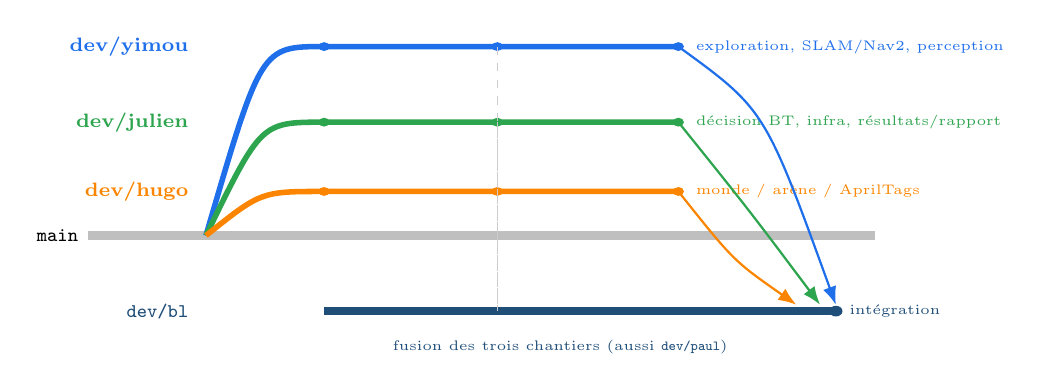
\begin{tikzpicture}[font=\scriptsize,xscale=1.0,yscale=0.8]
  \draw[gray!50,line width=3pt] (0,0) -- (10,0); \node[left] at (0,0){\texttt{main}};
  % feature branches
  \foreach \y/\name/\c in {3.0/{dev/yimou}/nccsky, 1.8/{dev/julien}/nccgreen, 0.7/{dev/hugo}/nccorange} {
     \draw[\c,line width=2pt] (1.5,0) .. controls (2.2,\y) .. (3.0,\y) -- (7.5,\y);
     \node[\c,left,font=\scriptsize\bfseries] at (1.4,\y) {\name};
     \fill[\c] (3.0,\y) circle (2pt); \fill[\c] (5.2,\y) circle (2pt); \fill[\c] (7.5,\y) circle (2pt);
  }
  \node[nccsky,right,font=\tiny] at (7.6,3.0){exploration, SLAM/Nav2, perception};
  \node[nccgreen,right,font=\tiny] at (7.6,1.8){décision BT, infra, résultats/rapport};
  \node[nccorange,right,font=\tiny] at (7.6,0.7){monde / arène / AprilTags};
  % bl integration branch
  \draw[nccblue,line width=3pt] (3.0,-1.2) -- (9.5,-1.2);
  \node[nccblue,left,font=\scriptsize\bfseries] at (1.4,-1.2){\texttt{dev/bl}};
  \node[nccblue,right,font=\tiny] at (9.55,-1.2){intégration};
  \foreach \y in {3.0,1.8,0.7} { \draw[dashed,gray!40] (5.2,\y) -- (5.2,-1.2); }
  \draw[-{Latex},nccsky,thick] (7.5,3.0) .. controls (8.6,2) .. (9.5,-1.1);
  \draw[-{Latex},nccgreen,thick] (7.5,1.8) .. controls (8.4,0.4) .. (9.3,-1.1);
  \draw[-{Latex},nccorange,thick] (7.5,0.7) .. controls (8.2,-0.4) .. (9.0,-1.1);
  \fill[nccblue] (9.5,-1.2) circle (2.4pt);
  \node[below,font=\tiny,nccblue] at (6,-1.5){fusion des trois chantiers (aussi \texttt{dev/paul})};
\end{tikzpicture}
\caption{Construction des branches : trois branches de fonctionnalités par développeur (chantiers issus
de l'historique git) sont fusionnées dans \texttt{dev/bl}, la branche d'intégration.}
\label{fig:branches}
\end{figure}

\noindent{\footnotesize\textbf{Répartition des tâches} (d'après l'historique git) :
\textbf{Yimou ZHANG} - exploration autonome, câblage SLAM/Nav2, cœur perception, benchmark ;
\textbf{Julien GIMENEZ} - décision Behavior-Tree \& orchestration en deux phases, infrastructure de
simulation (WSL/GPU/RTF/DDS), résultats, intégration (\texttt{bl}) et rapport ;
\textbf{Hugo FANCHINI} - monde de simulation, arène de sauvetage et placement des cibles AprilTag
(\texttt{rescue\_world}) ;
\textbf{Paul CINTRA} - support et tests perception/détection (\texttt{dev/paul}).}

% =================== 6. RESULTS ===================
\section{Résultats}
La Fig.~\ref{fig:seq} montre les algorithmes RViz en direct au fil de la mission ; la
Fig.~\ref{fig:results} les artefacts livrables. Tous proviennent de l'unique run final
(\texttt{results/examples/l18\_nominal}). Une démonstration vidéo de la mission complète est disponible : \url{https://www.youtube.com/watch?v=BKXprWFloFs}.

\begin{figure}[htbp]
\centering
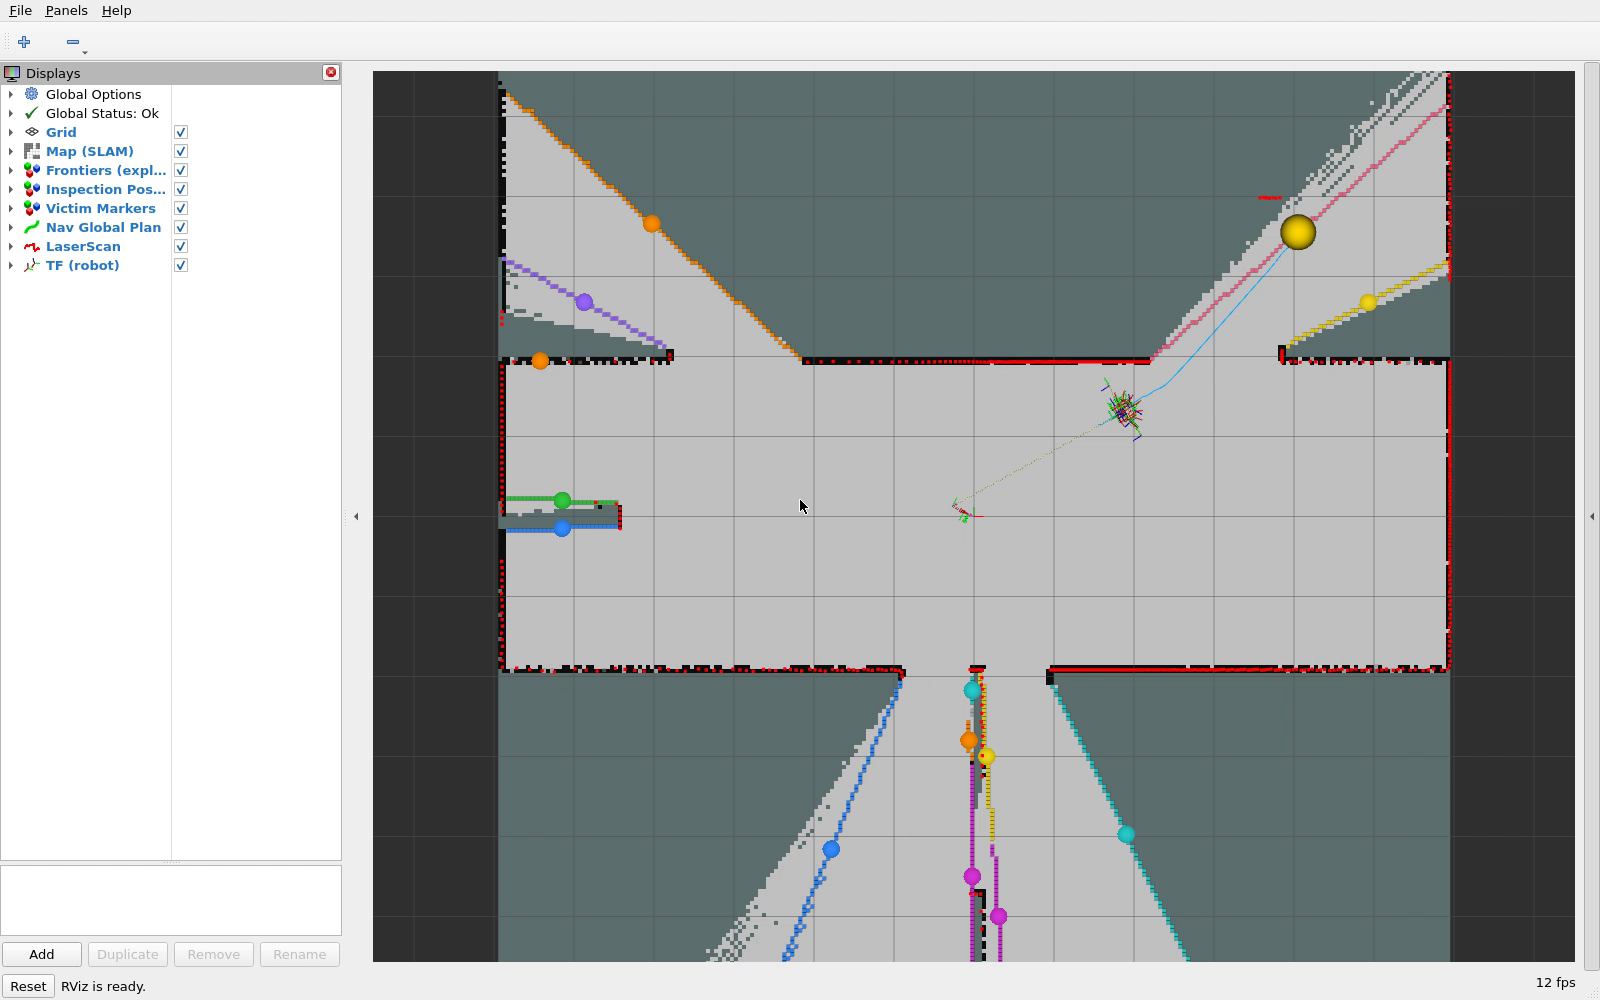
\includegraphics[width=0.315\linewidth]{rviz_seq_1}\hfill
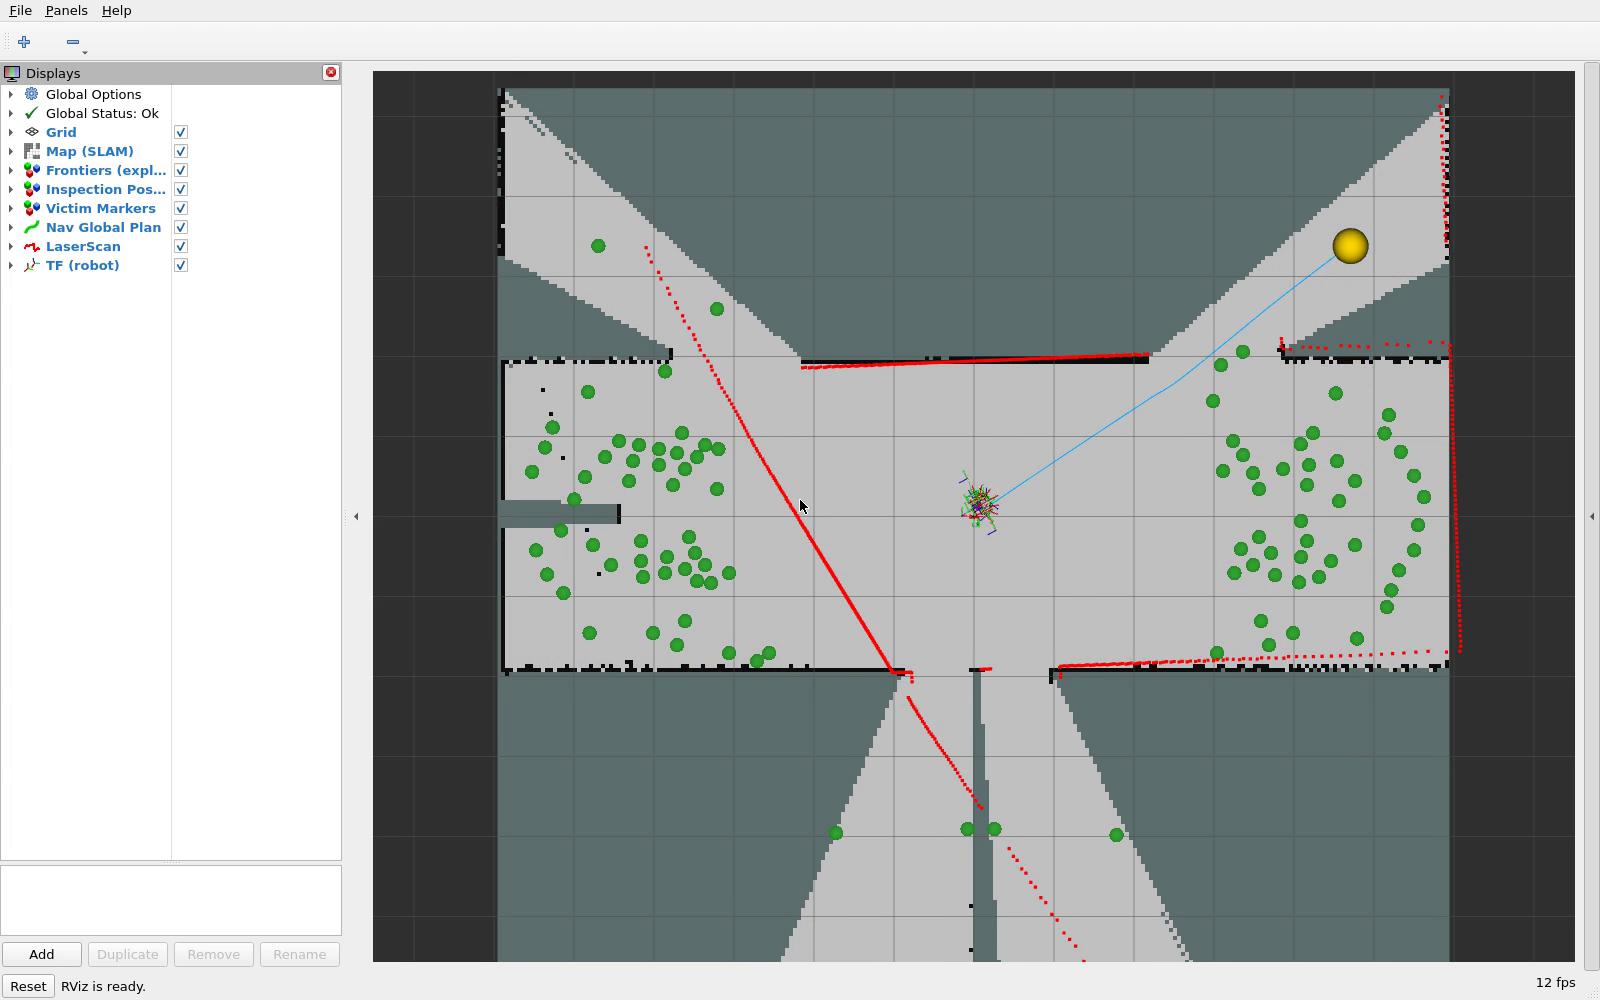
\includegraphics[width=0.315\linewidth]{rviz_seq_2}\hfill

\includegraphics[width=0.315\linewidth]{rviz_seq_3}\\[3pt]
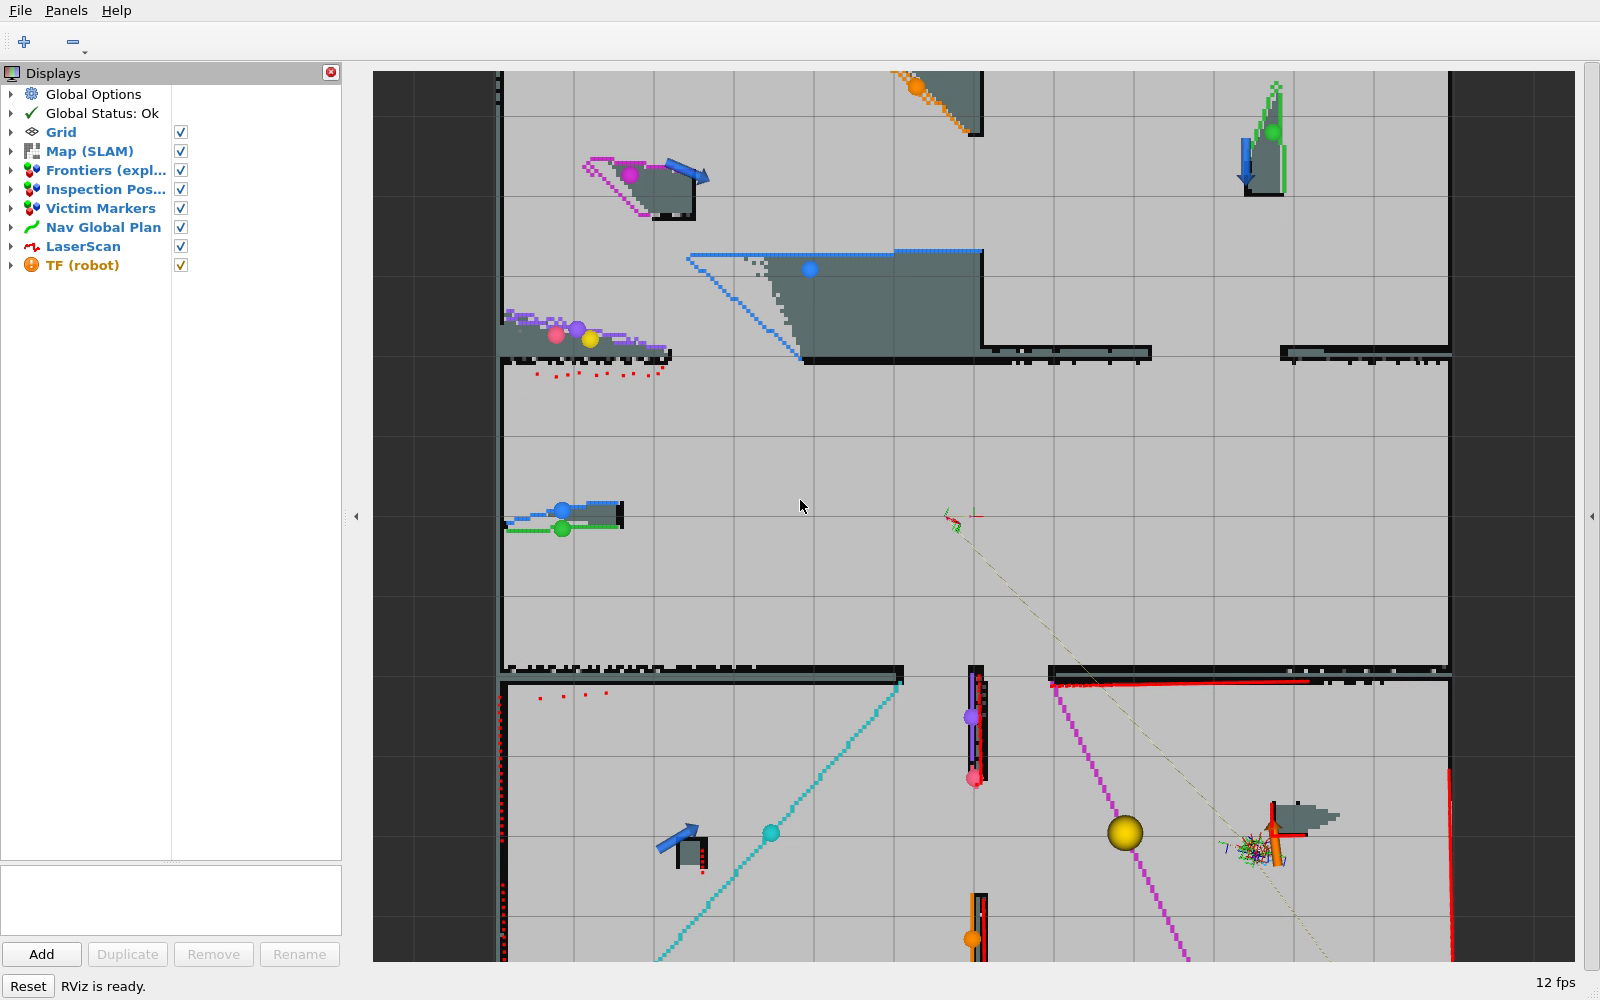
\includegraphics[width=0.315\linewidth]{rviz_seq_4}\hfill

\includegraphics[width=0.315\linewidth]{rviz_seq_5}\hfill
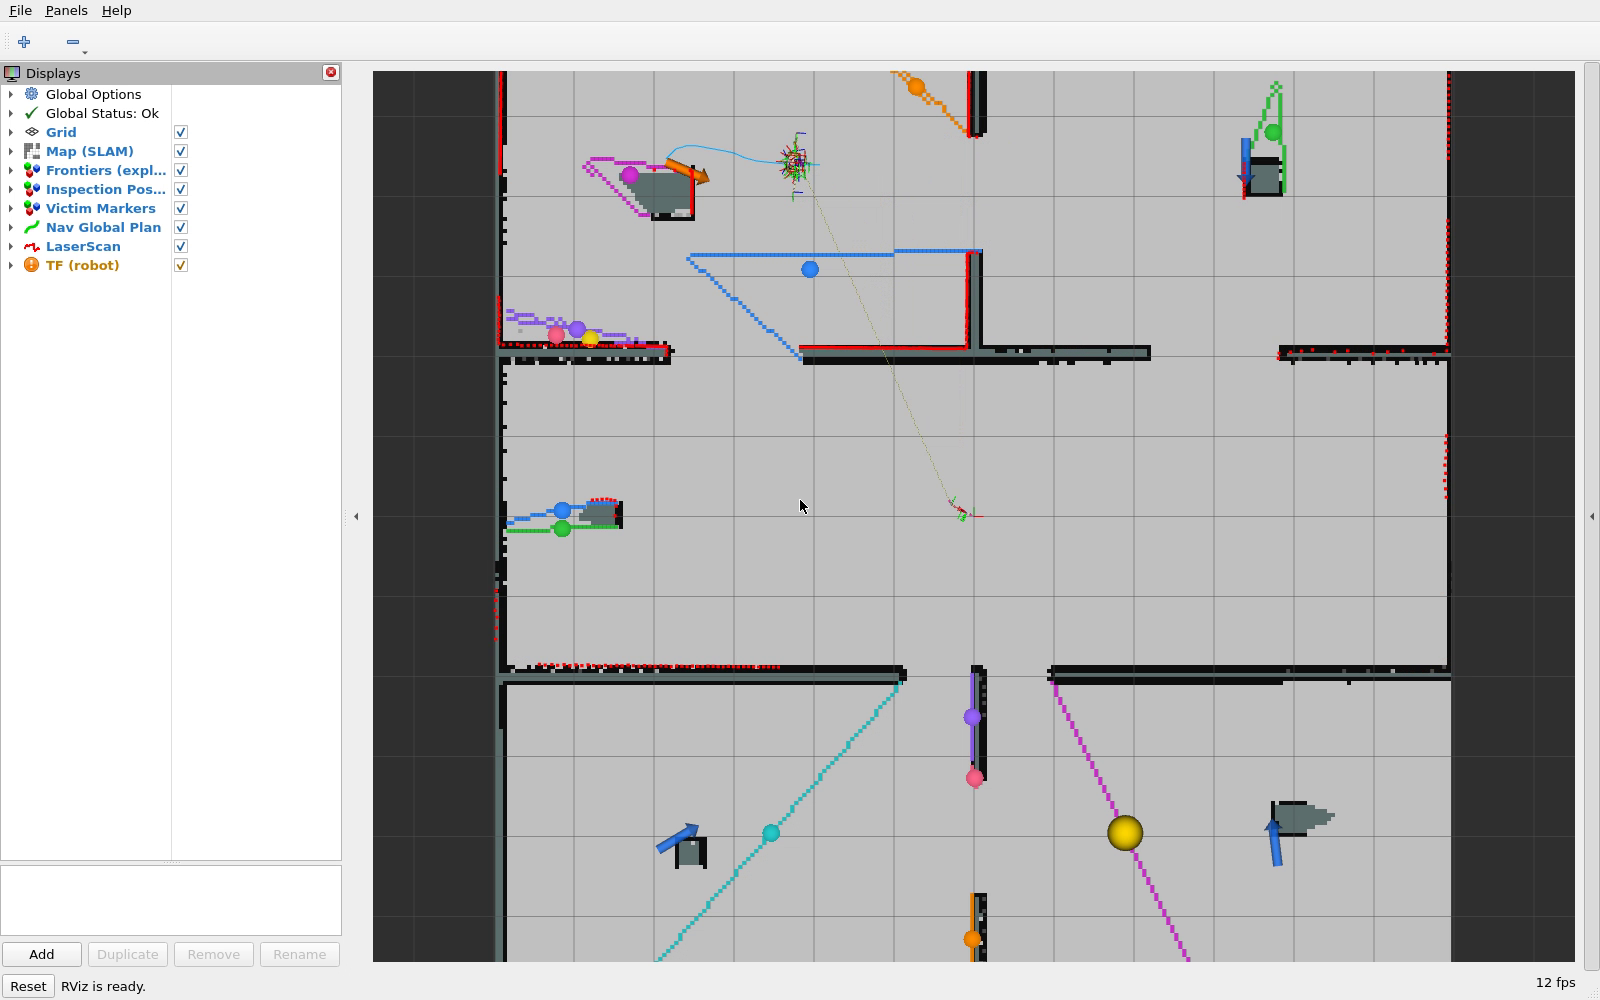
\includegraphics[width=0.315\linewidth]{rviz_seq_6}
\caption{RViz en direct à six moments clés (1--3 : exploration précoce, carte presque construite,
transition de phase ; 4--6 : inspection des pièces, victimes apparaissant, carte finale) - montrant la
carte (SLAM), les frontières, les poses d'inspection, le plan Nav2, le LaserScan et les quatre marqueurs
de victimes. Capturé en HD sur un serveur X virtuel.}
\label{fig:seq}
\end{figure}

\begin{figure}[htbp]
\centering
\begin{subfigure}{0.33\linewidth}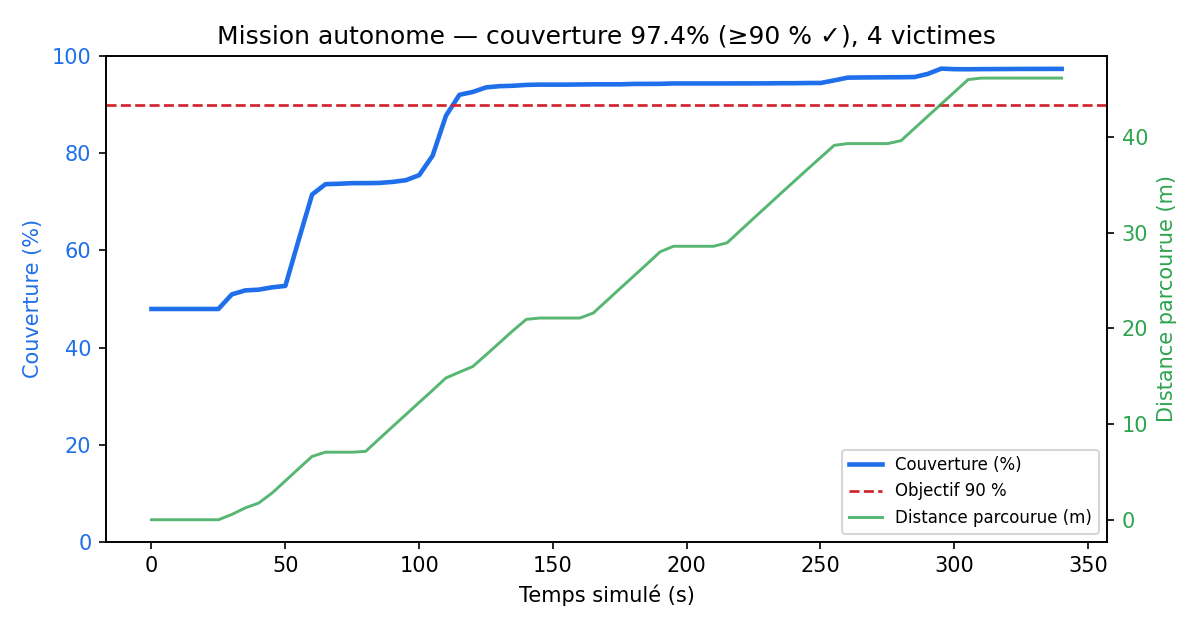
\includegraphics[width=\linewidth]{coverage_curve}\caption{Couverture \& chemin en fonction du temps (cible 90\,\%).}\end{subfigure}\hfill
\begin{subfigure}{0.33\linewidth}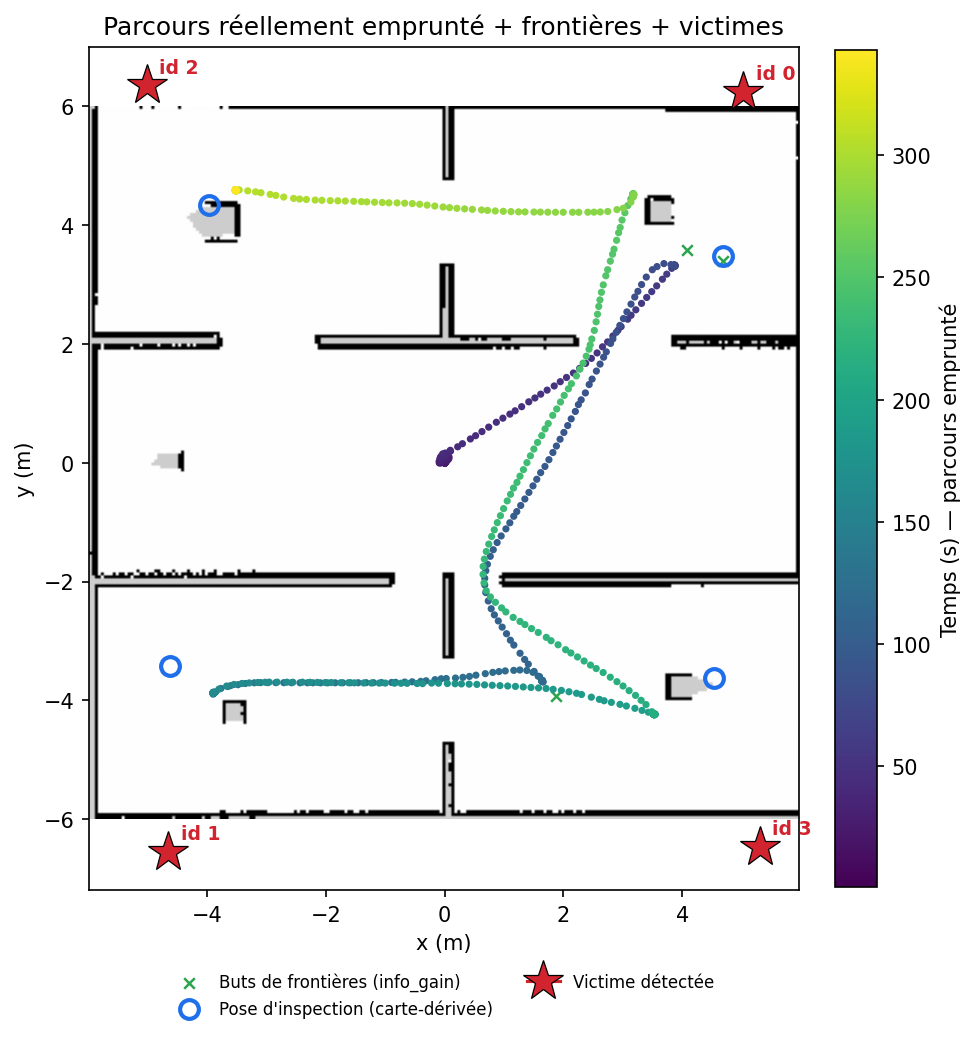
\includegraphics[width=\linewidth]{trajectory_map}\caption{Chemin réel (coloré dans le temps), se faufilant par les embrasures.}\end{subfigure}\hfill
\begin{subfigure}{0.32\linewidth}
\includegraphics[width=\linewidth]{mission_map}\caption{Carte finale : 4 victimes + tournée d'inspection.}\end{subfigure}
\caption{Résultats quantitatifs : \textbf{97,35\,\%} de couverture et \textbf{4/4} victimes, entièrement
autonome. La trajectoire est le chemin réel dans le repère carte ; les murs sont dessinés par-dessus, si
bien qu'elle passe visiblement par les embrasures (vérifié : aucun segment ne traverse un mur).}
\label{fig:results}
\end{figure}

\begin{figure}[htbp]
\centering
\begin{subfigure}{0.49\linewidth}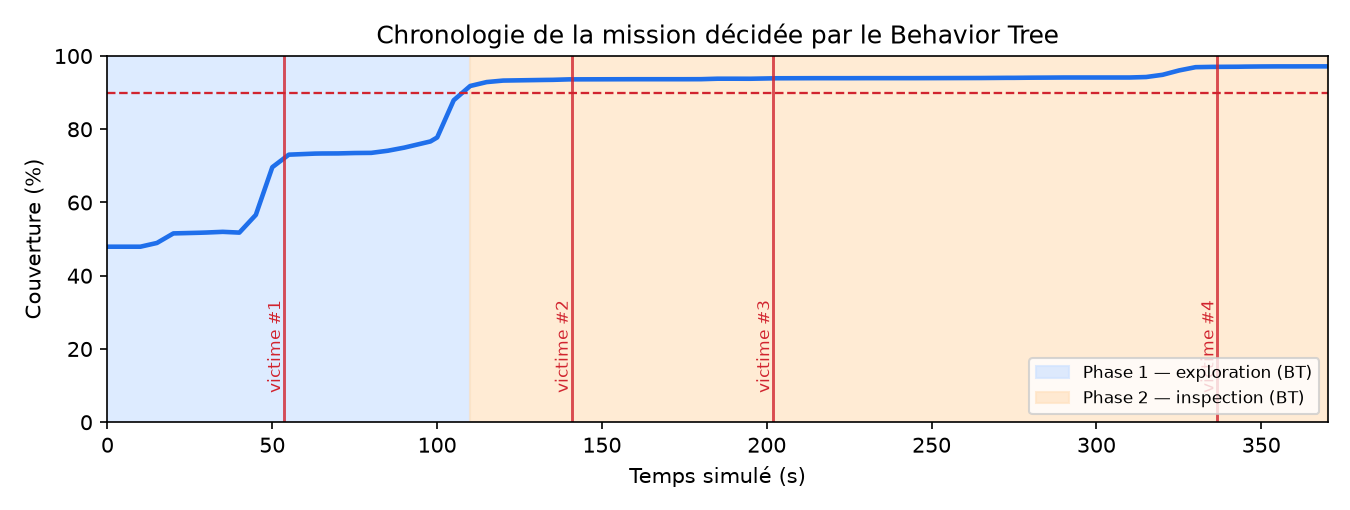
\includegraphics[width=\linewidth]{mission_timeline}\caption{Chronologie décidée par le BT : bandes Phase~1 (bleu) / Phase~2 (orange) et l'instant de détection de chaque victime.}\end{subfigure}\hfill
\begin{subfigure}{0.30\linewidth}
\includegraphics[width=\linewidth]{annotated_map_hd}\caption{Livrable : carte finale annotée des victimes.}\end{subfigure}\hfill
\begin{subfigure}{0.185\linewidth}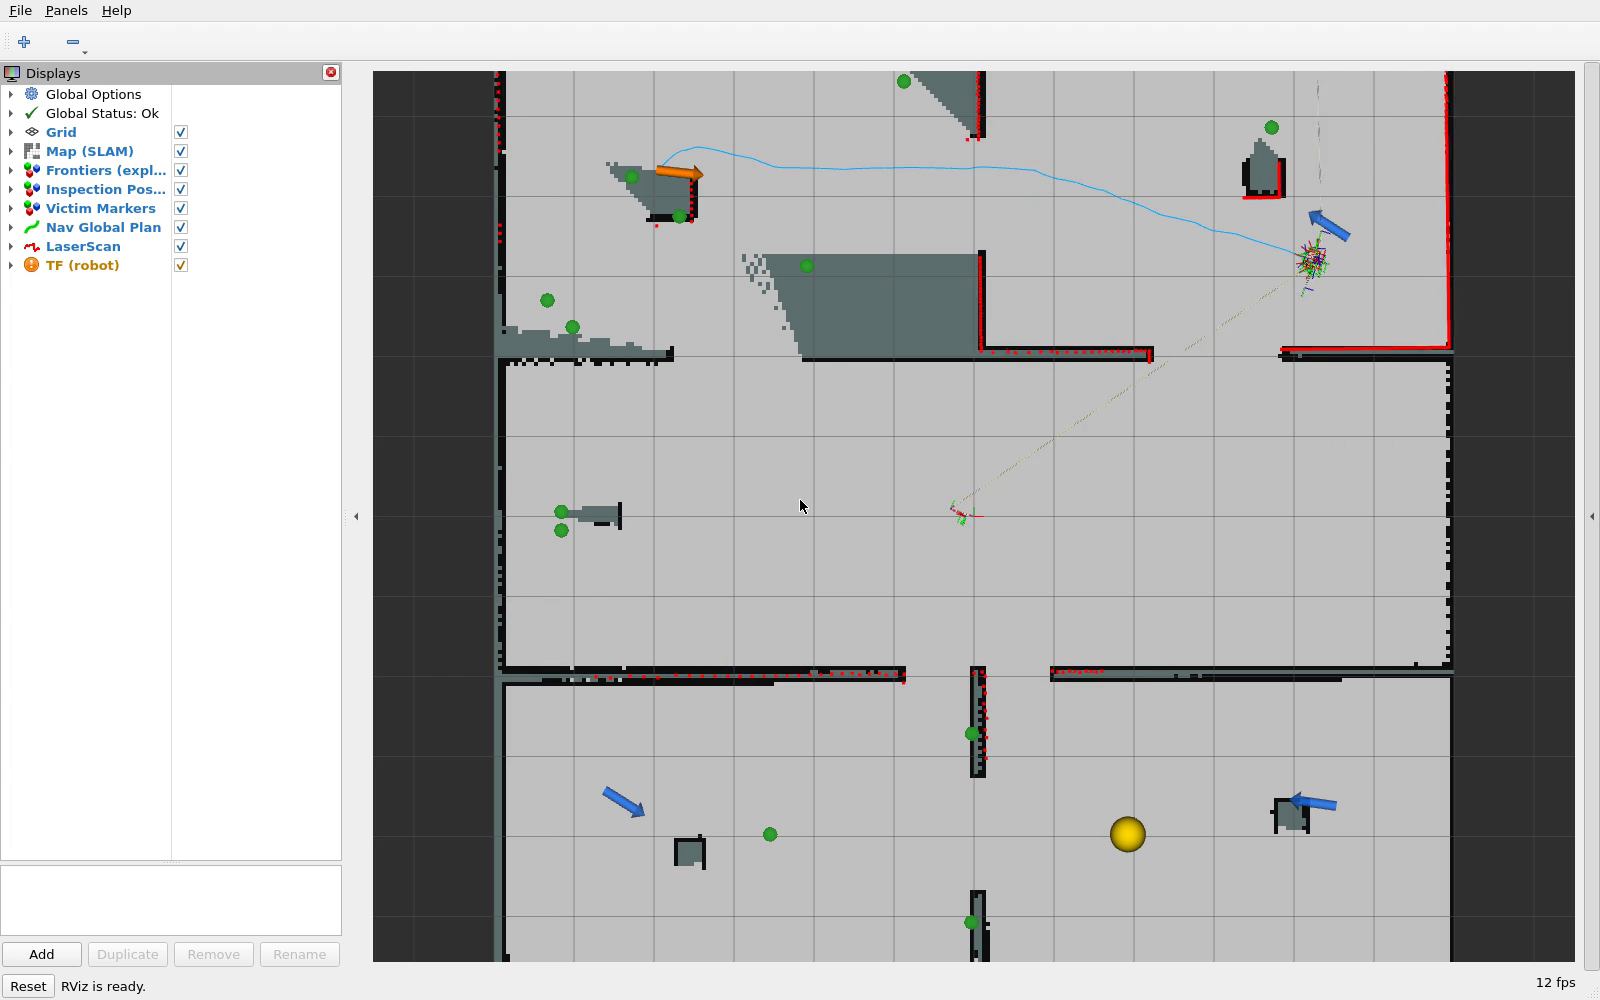
\includegraphics[width=\linewidth]{rviz_live}\caption{RViz en direct.}\end{subfigure}
\caption{Chronologie de la mission et le livrable de l'énoncé («~carte finale annotée de toutes les
positions des victimes~»). La séparation des phases et les instants de détection confirment
l'orchestration par le BT.}
\label{fig:timeline}
\end{figure}

\begin{figure}[htbp]
\centering

\includegraphics[width=0.92\linewidth]{mission_summary}
\caption{Montage de synthèse en un coup d'œil : carte finale avec les quatre victimes et la tournée
d'inspection (en haut à gauche), la trajectoire réelle colorée dans le temps (en haut à droite), la
couverture et la longueur du chemin au fil du temps (en bas à gauche) et la carte annotée livrable (en
bas à droite). Tout est régénéré à partir de l'unique run archivé, de sorte que les figures sont
reproductibles à partir des données.}
\label{fig:montage}
\end{figure}

\head{Lecture des résultats.} La courbe de couverture (Fig.~\ref{fig:results}a) montre clairement les
deux phases : une montée rapide pendant l'exploration jusqu'à la cible de 90\,\%, puis un plateau pendant
l'inspection tandis que la longueur du chemin continue de croître (le robot se déplace encore, de pièce en
pièce, mais la carte est déjà complète). La chronologie de mission (Fig.~\ref{fig:timeline}a) superpose
les quatre instants de détection des victimes sur les bandes de phase : les premières victimes sont
attrapées \emph{pendant} l'exploration lorsque le robot passe par hasard près d'un tag mural, et les
restantes \emph{pendant} l'inspection - exactement le comportement que prédit la conception en deux
phases. La trajectoire (Fig.~\ref{fig:results}b) confirme que le robot visite les quatre pièces et
revient, en se faufilant par chaque embrasure.

\head{Exécution et reproductibilité.} Toute la pile démarre d'une seule commande,
\texttt{ros2 launch rescue\_bringup bringup\_tb4.launch.py}. Le run nominal est archivé
(\texttt{results/examples/l18\_nominal}) de sorte que chaque figure de ce rapport soit régénérable à
partir des données ; le benchmark bonus est \emph{reprenable} (chaque run persiste son résumé, les runs
valides sont sautés au redémarrage), ce qui a permis à la campagne de survivre aux redémarrages de
l'hôte. RViz est capturé en vidéo HD sur une machine sans écran via un serveur X virtuel, donnant la
séquence d'algorithmes en direct de la Fig.~\ref{fig:seq}.

% =================== 7. LESSONS + TIMELINE ===================
\section{Enseignements tirés et calendrier}
\head{Enseignements tirés.} Quatre leçons ressortent, et elles tiennent autant de la méthode d'ingénierie
que de la robotique. La première est de \emph{mesurer avant de prescrire}. Deux fois nous étions certains
de savoir pourquoi la machine hôte redémarrait sans cesse - ce devait être la mémoire, puis sûrement une
mise à jour Windows en attente - et deux fois nous avions tort ; seuls le journal d'événements,
\texttt{free} et \texttt{nvidia-smi} ont désigné les vrais coupables, un plantage thermique du pilote GPU
et, séparément, un renderer caméra affamé par un facteur temps réel effondré alors que ses métadonnées
continuaient de circuler et masquaient le problème. La deuxième leçon est qu'\emph{un correctif révèle le
suivant} : passer de zéro à quatre victimes a signifié éplucher six causes empilées - un objectif non
cartographié, un objectif sur un mur, un réflexe de sécurité, un coin inatteignable, un routage
inter-pièces fragile et enfin la caméra affamée - où chaque correction ne faisait qu'exposer celle d'en
dessous. La troisième est que \emph{le robuste l'emporte sur le rigide} : dans une arène cloisonnée, un
explorateur adaptatif qui visite déjà chaque pièce, suivi d'un balayage caméra complet à 360$^\circ$,
bat systématiquement une patrouille par points de passage écrite à la main qui se casse dès que la carte
diffère légèrement. Et la quatrième est la \emph{conformité par conception} - en faisant véritablement
\emph{orchestrer} la mission par le Behavior Tree plutôt que de la simplement surveiller, nous satisfaisons
l'exigence «~décision par BT, pas de FSM~» de l'énoncé dans l'esprit et pas seulement sur le papier.

\head{Calendrier (L13--L18).} Le projet a suivi le calendrier suggéré (Fig.~\ref{fig:timelineL}).

\begin{figure}[htbp]
\centering
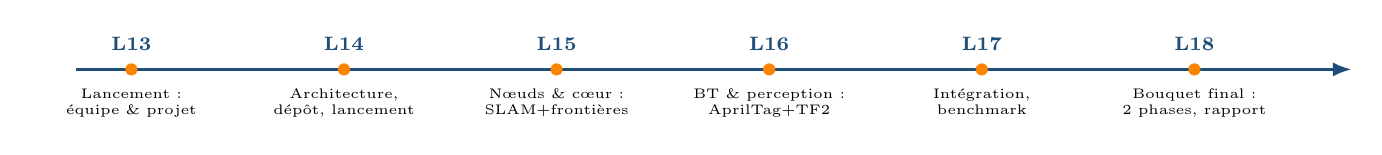
\begin{tikzpicture}[font=\scriptsize]
  \draw[line width=1.2pt,nccblue,-{Latex[length=2.4mm]}] (0,0) -- (16.2,0);
  \foreach \x/\l/\d in {0.3/L13/{Lancement :\\équipe \& projet}, 3/L14/{Architecture,\\dépôt, lancement}, 5.7/L15/{Nœuds \& cœur :\\SLAM+frontières}, 8.4/L16/{BT \& perception :\\AprilTag+TF2}, 11.1/L17/{Intégration,\\benchmark}, 13.8/L18/{Bouquet final :\\2 phases, rapport}} {
     \fill[nccorange] (\x+0.4,0) circle (2.2pt);
     \node[above,nccblue,font=\scriptsize\bfseries] at (\x+0.4,0.12){\l};
     \node[below,align=center,font=\tiny,text width=24mm] at (\x+0.4,-0.12){\d};
  }
\end{tikzpicture}
\caption{Les six séances L13--L18 et leurs jalons.}
\label{fig:timelineL}
\end{figure}

\section{Discussion et conclusion}
Avec le recul, le projet réussit moins grâce à un quelconque algorithme astucieux que grâce à la manière
dont les pièces sont amenées à coopérer. L'exploration est une recherche de frontières de manuel, le
planificateur et le contrôleur sont des plugins Nav2 standard, le SLAM est \texttt{slam\_toolbox} prêt à
l'emploi, et le détecteur est \texttt{apriltag\_ros} ; ce que nous avons apporté, c'est l'\emph{intégration}
- un Behavior Tree qui transforme ces composants indépendants en une mission cohérente, et une seconde
phase autonome qui comble l'écart entre «~la carte est complète~» et «~chaque victime est trouvée~». C'est
exactement le glissement que demande l'énoncé : passer de l'écriture d'un code qui se contente de tourner
à l'ingénierie d'un système dont les parties tiennent ensemble en conditions réelles.

La conception en deux phases est le cœur conceptuel du résultat. Un robot qui se contente d'explorer va,
dans un bâtiment cloisonné, cartographier confortablement chaque pièce depuis son embrasure avec un LIDAR
de douze mètres et n'aura jamais besoin d'y entrer - ce qui est efficace pour la cartographie mais fatal
pour une caméra qui ne voit un tag qu'à deux mètres. Séparer la \emph{cartographie} de l'\emph{inspection},
et déduire les poses d'inspection de la carte que le robot vient de construire plutôt que d'une connaissance
préalable des victimes, garde le système entièrement autonome tout en rendant la détection fiable. Le
Behavior Tree est ce qui rend cette séparation nette : chaque phase est un nœud qui s'exécute jusqu'à sa
propre condition de succès, et la mission se lit simplement comme une séquence.

La robustesse, enfin, fut une leçon en soi. Un run qui marche sur une machine n'est pas la même chose
qu'un système qui marche : un costmap légèrement différent sur l'ordinateur d'un coéquipier suffisait à
rendre deux poses d'inspection inatteignables, jusqu'à ce que l'inspecteur apprenne à attendre que le
costmap se stabilise et à se rabattre sur une pose tirée vers l'intérieur de la pièce. La conclusion
honnête de ce projet porte donc autant sur la méthode - mesurer, isoler une cause à la fois, rendre le
système tolérant plutôt que rigide - que sur les chiffres finaux. Les prochaines étapes naturelles
seraient de comparer A* à NavFn sur un costmap moins agressif, d'essayer un contrôleur Regulated Pure
Pursuit pour des traversées d'embrasures plus douces, et d'ajouter un second robot en laissant le
Behavior Tree coordonner une carte partagée.

\section*{Remerciements}
Nous remercions chaleureusement \textbf{Zhi Yan}, enseignant-chercheur à l'ENSTA, pour le module IA712 et
l'encadrement qui ont rendu ce projet possible.

% =================== REFERENCES ===================
\renewcommand{\refname}{Références}
\begingroup
\small
\begin{thebibliography}{99}
\setlength{\itemsep}{0pt}
\bibitem{assign} IA712 Mobile Robotics - Final Project, Project~B (énoncé). Site : \url{https://yzrobot.github.io/IA712/}.
\bibitem{yamauchi} B.~Yamauchi, \emph{A frontier-based approach for autonomous exploration}, IEEE CIRA, 1997.
\bibitem{stachniss} C.~Stachniss et al., \emph{Information gain-based exploration using Rao-Blackwellized particle filters}, ICRA, 2005.
\bibitem{slamtb} S.~Macenski, I.~Jambrecic, \emph{slam\_toolbox: SLAM for the dynamic world}, JOSS, 2021.
\bibitem{nav2} S.~Macenski et al., \emph{The Marathon~2: A navigation system (Nav2)}, IROS, 2020.
\bibitem{btcpp} D.~Faconti et al., \emph{BehaviorTree.CPP} library, \url{https://www.behaviortree.dev/}.
\bibitem{apriltag} E.~Olson, \emph{AprilTag: A robust and flexible visual fiducial system}, ICRA, 2011; \texttt{apriltag\_ros}.
\bibitem{tf2} T.~Foote, \emph{tf2: The transform library}, IEEE TePRA, 2013.
\bibitem{cm} IA712 Mobile Robotics - supports de référence, \url{https://yzrobot.github.io/IA712/}.
\bibitem{repo} Project repository, \url{https://github.com/YiZeems/autonomous-search-and-rescue}.
\end{thebibliography}
\endgroup

\end{document}
